% Options for packages loaded elsewhere
\PassOptionsToPackage{unicode}{hyperref}
\PassOptionsToPackage{hyphens}{url}
\documentclass[
  11pt,
]{article}
\usepackage{xcolor}
\usepackage[margin=22mm]{geometry}
\usepackage{amsmath,amssymb}
\setcounter{secnumdepth}{-\maxdimen} % remove section numbering
\usepackage{iftex}
\ifPDFTeX
  \usepackage[T1]{fontenc}
  \usepackage[utf8]{inputenc}
  \usepackage{textcomp} % provide euro and other symbols
\else % if luatex or xetex
  \usepackage{unicode-math} % this also loads fontspec
  \defaultfontfeatures{Scale=MatchLowercase}
  \defaultfontfeatures[\rmfamily]{Ligatures=TeX,Scale=1}
\fi
\usepackage{lmodern}
\ifPDFTeX\else
  % xetex/luatex font selection
\fi
% Use upquote if available, for straight quotes in verbatim environments
\IfFileExists{upquote.sty}{\usepackage{upquote}}{}
\IfFileExists{microtype.sty}{% use microtype if available
  \usepackage[]{microtype}
  \UseMicrotypeSet[protrusion]{basicmath} % disable protrusion for tt fonts
}{}
\makeatletter
\@ifundefined{KOMAClassName}{% if non-KOMA class
  \IfFileExists{parskip.sty}{%
    \usepackage{parskip}
  }{% else
    \setlength{\parindent}{0pt}
    \setlength{\parskip}{6pt plus 2pt minus 1pt}}
}{% if KOMA class
  \KOMAoptions{parskip=half}}
\makeatother
\usepackage{graphicx}
\makeatletter
\newsavebox\pandoc@box
\newcommand*\pandocbounded[1]{% scales image to fit in text height/width
  \sbox\pandoc@box{#1}%
  \Gscale@div\@tempa{\textheight}{\dimexpr\ht\pandoc@box+\dp\pandoc@box\relax}%
  \Gscale@div\@tempb{\linewidth}{\wd\pandoc@box}%
  \ifdim\@tempb\p@<\@tempa\p@\let\@tempa\@tempb\fi% select the smaller of both
  \ifdim\@tempa\p@<\p@\scalebox{\@tempa}{\usebox\pandoc@box}%
  \else\usebox{\pandoc@box}%
  \fi%
}
% Set default figure placement to htbp
\def\fps@figure{htbp}
\makeatother
\usepackage{svg}
\setlength{\emergencystretch}{3em} % prevent overfull lines
\providecommand{\tightlist}{%
  \setlength{\itemsep}{0pt}\setlength{\parskip}{0pt}}
\usepackage{bookmark}
\IfFileExists{xurl.sty}{\usepackage{xurl}}{} % add URL line breaks if available
\urlstyle{same}
\hypersetup{
  hidelinks,
  pdfcreator={LaTeX via pandoc}}

\author{}
\date{}

\begin{document}

\section{Two measuring scales, one Weyl
product}\label{two-measuring-scales-one-weyl-product}

Two symbols can have different derivative scales. Their Weyl product
couples those scales through the symplectic form. The useful parameter
measures the coupling; it need not control either scale separately. We
identify the exact compatibility conditions, derive the quantization
formula, and prove product and remainder estimates.

\href{metric-localization.pdf}{Localizing symbols with moving metrics}
supplies symbol spaces, partitions and bounded compactly supported
approximation. \href{gauss-transform-estimates.pdf}{Quadratic Fourier
multipliers at a moving scale} supplies the Fourier estimates with
convention \(D=-i\partial\). We also use finite-dimensional linear
algebra; completeness, compact smooth approximation and integration in
\(L^2\); and the tempered Schwartz kernel theorem: every continuous
linear map \(\mathcal S(V)\to\mathcal S'(V)\) has a unique kernel in
\(\mathcal S'(V\times V)\). The kernel theorem is used only for the
converse description of all Schwartz-to-distribution operators. Sections
4.1--4.5 below prove that theorem with the original Schwartz seminorms
and continuity into the strong dual. The operators and kernel identities
needed for the product are constructed directly. Basic references are
{[}Lerner, Metrics in phase space{]}.

Throughout, \(V\) is a real vector space of dimension \(n\geq1\),
\(W=V\oplus V^*\), and \[
\sigma((x,\xi),(y,\eta))=\langle\xi,y\rangle-\langle x,\eta\rangle.
\tag{W1}
\] Measures on \(V\) and \(V^*\) are dual for Fourier inversion with
coefficient \((2\pi)^{-n}\). Multiplying one measure by a positive
constant divides the other by that constant; the phase-space measure and
all quantizations below are unchanged.

\subsection{1. Quadratic forms and the cross
parameter}\label{quadratic-forms-and-the-cross-parameter}

For a positive-definite quadratic form \(q\) on \(W\), define \[
q^\sigma(T)=\sup_{S\ne0}\frac{|\sigma(T,S)|^2}{q(S)}.
\tag{W2}
\] This is positive definite. Ordinary quadratic duality, composed with
the invertible linear map induced by \(\sigma\), gives \[
(q^\sigma)^\sigma=q,\qquad (c q)^\sigma=c^{-1}q^\sigma,
\qquad q\leq C r\ \Longleftrightarrow\ r^\sigma\leq Cq^\sigma.
\tag{W3}
\] For example, write \(q(T)=T^tQT\) in coordinates and let \(J\)
represent \(\sigma\). Then \(q^\sigma(T)=T^tJQ^{-1}J^tT\); substitution
proves the first identity, and inversion of positive matrices proves the
order reversal. Alternatively, all three follow by mapping the unit
ellipsoid to its polar ellipsoid and using that taking the polar twice
returns the original ellipsoid.

We will need an exact formula for the dual of a sum. If \(F_1,F_2\) are
positive quadratic forms on a finite-dimensional space and primes denote
ordinary dual forms, then \[
(F_1+F_2)'(\zeta)
=\min_{\zeta_1+\zeta_2=\zeta}
\big(F_1'(\zeta_1)+F_2'(\zeta_2)\big).
\tag{W4}
\] To prove it, represent the forms by positive matrices \(A_1,A_2\).
Put \(v=(A_1+A_2)^{-1}\zeta\) and \(\zeta_j=A_jv\). Every other
decomposition is \((\zeta_1+e,\zeta_2-e)\). Expanding its objective
gives the value \(v^t(A_1+A_2)v\), plus \(e^t(A_1^{-1}+A_2^{-1})e\); the
mixed terms cancel. The latter quantity is nonnegative and vanishes only
at \(e=0\). This proves both the minimum and its value. In particular,
if \(g=(g_1+g_2)/2\), \[
g^\sigma(T)=2\min_{T_1+T_2=T}
\big(g_1^\sigma(T_1)+g_2^\sigma(T_2)\big).
\tag{W5}
\] The factor two comes from the factor one half in the mean; it is not
optional.

At one point of phase space, set \[
h_j^2=\sup_{T\ne0}\frac{g_j(T)}{g_j^\sigma(T)},\qquad
H^2=\sup_{T\ne0}\frac{g_1(T)}{g_2^\sigma(T)}
=\sup_{T\ne0}\frac{g_2(T)}{g_1^\sigma(T)}.
\tag{W6}
\] The two expressions for \(H\) are equal by (W3): each is the least
constant in one of the equivalent inequalities
\(g_1\leq H^2g_2^\sigma\), \(g_2\leq H^2g_1^\sigma\). These are also
equivalent to \[
|\sigma(T,S)|^2\leq H^2g_1^\sigma(T)g_2^\sigma(S).
\tag{W7}
\] Indeed, divide by \(g_2^\sigma(S)\), take the supremum over \(S\),
and use (W3).

For the mean metric, write \(h_g^2=\sup g/g^\sigma\). Then \[
\max(h_1^2,h_2^2,H^2)\leq4h_g^2
\leq h_1^2+h_2^2+2H^2.
\tag{W8}
\] For the first inequality, \(g_j\leq2g\) and
\(g^\sigma\leq2g_k^\sigma\) show that
\(g_j(T)/g_k^\sigma(T)\leq4g(T)/g^\sigma(T)\), for both choices of
\(j,k\). For the second, \(2g=g_j+g_k\leq(h_j^2+H^2)g_j^\sigma\).
Dualizing gives \(2g_j\leq(h_j^2+H^2)g^\sigma\). Add the two
inequalities. No uncertainty inequality has been assumed in this
argument.

\subsection{2. Transport between compatible
metrics}\label{transport-between-compatible-metrics}

Let \(g_1,g_2\) be slowly varying metrics on \(W\), in the sense of
\href{metric-localization.pdf}{Localizing symbols with moving metrics}.
Write \(q_j(X)=g_{j,X}^\sigma\). Each metric is assumed symplectically
temperate, meaning that for fixed constants \(C,N\), uniformly in
\(X,Y,T\), \[
q_j(X)(T)\leq Cq_j(Y)(T)
\big(1+q_j(Y)(X-Y)\big)^N.
\tag{W9}
\] By (W3), this is equivalent to the primal inequality
\(g_{j,Y}\leq Cg_{j,X}(1+q_j(Y)(X-Y))^N\). Constants can be enlarged so
that a common \(C\geq1\), \(N\geq0\) works for both metrics. The bases
of the quadratic distances matter.

The cross tests are \[
\begin{split}
q_1(X)(T)&\leq Cq_1(Y)(T)
\big(1+q_2(X)(Y-X)\big)^N,\\
q_2(X)(T)&\leq Cq_2(Y)(T)
\big(1+q_1(X)(Y-X)\big)^N.
\end{split}
\tag{W10}
\] We call the pair compatible when these hold. They require more than
temperateness of each metric separately.

\textbf{Lemma 2.1 (metric transport).} Under (W9)--(W10), there are
common constants \(C,L\) such that, for all \(j,k\in\{1,2\}\), \[
q_j(X)\leq Cq_j(Y)\big(1+q_k(Y)(X-Y)\big)^L,
\quad
g_{j,Y}\leq Cg_{j,X}\big(1+q_k(Y)(X-Y)\big)^L.
\tag{W11}
\] Moreover, with \(g=(g_1+g_2)/2\), there are \(C',L'\) such that \[
g_{j,Y}\leq C'g_{j,X}
\big(1+g_Y^\sigma(X-Y)\big)^{L'},\qquad j=1,2.
\tag{W12}
\] Consequently \(g\) is symplectically temperate.

\textbf{Proof.} For \(j=k\), the first estimate in (W11) is (W9). For
\(j\ne k\), (W9) gives \[
1+q_k(X)(X-Y)\leq C_0\big(1+q_k(Y)(X-Y)\big)^{N+1}.
\] Insert this into (W10). Dualizing gives the second estimate in (W11).

Fix \(X,Y\), choose any intermediate point \(Z\), and put \[
R=1+q_1(Y)(X-Z)+q_2(Y)(Z-Y).
\] Use (W11) first on the segment from \(Z\) to \(Y\), with \(k=2\). It
gives \[
g_{j,Y}\leq Cg_{j,Z}R^L,
\qquad q_1(Z)(X-Z)\leq Cq_1(Y)(X-Z)R^L\leq CR^{L+1}.
\] Use (W11) again on the segment from \(X\) to \(Z\), now with \(k=1\).
Thus \[
g_{j,Z}\leq Cg_{j,X}(1+q_1(Z)(X-Z))^L
\leq C_1g_{j,X}R^{L(L+1)}.
\] Multiplication gives an exponent \(L^2+2L\). Minimize \(R\) using
(W5); its minimum is \(1+g_Y^\sigma(X-Y)/2\). This proves (W12). Adding
the two primal inequalities proves temperateness of the mean. It is also
slowly varying: if \(g_X(Y-X)\) is sufficiently small, then
\(g_{j,X}(Y-X)\leq2g_X(Y-X)\) is small for both metrics, and their
slow-variation comparisons can be added. \(\square\)

A positive weight \(m\) is symplectically temperate for \(g\) if it is
\(g\)-continuous locally and \[
m(Y)\leq Cm(X)\big(1+g_Y^\sigma(X-Y)\big)^N.
\tag{W13}
\] Its reciprocal has the same property, with possibly larger exponent.
In fact, apply (W13) with \(X,Y\) exchanged and use (W9) to replace the
resulting distance based at \(X\) by a power of the distance based at
\(Y\). Local comparability also reverses. Products and positive real
powers are handled in the same way.

Suppose \(m_j\) is initially temperate for its own \(g_j\). The
additional weight tests are \[
m_1(Y)\leq Cm_1(X)(1+q_2(X)(X-Y))^N,
\quad
m_2(Y)\leq Cm_2(X)(1+q_1(X)(X-Y))^N.
\tag{W14}
\] For a compatible pair, these are equivalent to both weights being
temperate for the mean \(g\). Here is the full reduction. Own
temperateness and (W14), with the distance-base conversion used above,
give \(m_j(Y)\leq Cm_j(X)(1+q_k(Y)(X-Y))^L\) for either \(k\). Repeat
the two-segment proof of (W12), replacing its primal metric factor by
\(m_j\); the estimate for \(q_1(Z)\) is unchanged. Minimization proves
(W13) for the mean. Local \(g\)-continuity follows from
\(g_j\)-continuity and \(g_j\leq2g\).

Conversely, \(g_Y^\sigma\leq2q_k(Y)\), followed by the distance-base
conversion for \(g_k\), turns mean temperateness into (W14). If only
mean temperateness and \(g_j\)-continuity were given at the outset, the
same inequality with \(k=j\) also proves own temperateness. This
explains the exact weight hypotheses used later.

\subsection{3. What the diagonal test
requires}\label{what-the-diagonal-test-requires}

On \(W\times W\), use the product metric and weight \[
G_{(Y,Z)}(T,S)=g_{1,Y}(T)+g_{2,Z}(S),\qquad
M(Y,Z)=m_1(Y)m_2(Z).
\tag{W15}
\] The product metric is slowly varying and the product weight is
locally \(G\)-continuous, directly from the separate local comparisons.

Use dual coordinates \((p,q;r,s)\) and the auxiliary quadratic phase
\(A_0(p,q;r,s)=2(q\cdot r-p\cdot s)\). Its symmetric map in the
convention of \href{gauss-transform-estimates.pdf}{Quadratic Fourier
multipliers at a moving scale} sends \((p,q;r,s)\) to \((-s,r;q,-p)\).
Substitution in that lesson's definition of the phase-dual form gives \[
G_{(Y,Z)}^{A_0}(T,S)=q_2(Z)(T)+q_1(Y)(S).
\tag{W16}
\] Consequently \(G_{(X,X)}\leq H(X)^2G_{(X,X)}^{A_0}\), and \(H(X)^2\)
is the least possible constant. Notice the interchange of the two
metrics in (W16).

\textbf{Theorem 3.1 (diagonal criterion).} The product metric is
uniformly \(A_0\)-temperate at the points \((X,X)\) if and only if (W10)
holds. If the individual weights are temperate for their own metrics,
the product weight is uniformly \(A_0,G\)-temperate there if and only if
(W14) holds.

\textbf{Proof of necessity.} In dual form, metric temperateness on the
diagonal says \[
q_1(X)(T)+q_2(X)(S)
\leq C\big(q_1(Y)(T)+q_2(Z)(S)\big)\mathcal D^L,
\quad
\mathcal D=1+q_2(Z)(X-Y)+q_1(Y)(X-Z).
\tag{W17}
\] Set \(Z=X,S=0\) to obtain the first cross test. Set \(Y=X,T=0\) for
the second. The analogous product-weight inequality is
\(m_1(Y)m_2(Z)\leq Cm_1(X)m_2(X)\mathcal D^L\). The same substitutions
and cancellation of a positive factor give (W14).

\textbf{Proof of sufficiency.} We supply the distance comparison that is
needed for this implication. For any single temperate metric \(g\),
write \(q(U)=g_U^\sigma\), and let \[
\mathcal E=1+q(Y)(X-Z)+q(Z)(X-Y),\qquad P=Y+Z-X.
\] Because \(P-Z=Y-X\) and \(P-Y=Z-X\), temperateness gives \[
q(P)(X-Y)\leq C\mathcal E^{L+1},\qquad
q(P)(X-Z)\leq C\mathcal E^{L+1}.
\] For example, the first is the comparison of \(q(P)\) with \(q(Z)\),
whose controlling distance \(P-Z\) is exactly \(-(X-Y)\). Compare
\(q(Y)\) with \(q(P)\); the controlling distance \(Y-P=X-Z\) is bounded
by the second estimate. Do the analogous comparison for \(q(Z)\). We
obtain \[
q(Y)(X-Y)+q(Z)(X-Z)\leq C'\mathcal E^{(L+1)^2}.
\tag{W18}
\]

Now take the mean metric from Section 2. Its dual is at most twice each
\(q_j\), so \(\mathcal E\leq2\mathcal D\). Apply (W12) to
\(g_{1,Y}/g_{1,X}\) and \(g_{2,Z}/g_{2,X}\), and then (W18). This yields
\[
g_{1,Y}(T)+g_{2,Z}(S)
\leq C''\big(g_{1,X}(T)+g_{2,X}(S)\big)\mathcal D^{L''}.
\] It is precisely the primal phase-temperateness condition from Section
5 of \href{gauss-transform-estimates.pdf}{Quadratic Fourier multipliers
at a moving scale}. Dualization gives (W17). The weights are temperate
for the mean by the preceding weight equivalence, so applying (W13) and
(W18) also proves the product-weight condition. \(\square\)

Taking \(g_1=g_2=g\) makes the cross tests consequences of ordinary
symplectic temperateness and its distance-base conversion. Thus one
temperate metric and any two temperate weights always satisfy the
diagonal conditions, with parameter \(H=h_g\). This includes metrics and
weights with no initial ordinary continuity.

\subsection{4. Kernels and the Weyl
normalization}\label{kernels-and-the-weyl-normalization}

For \(a\in\mathcal S(W)\) and \(\tau\in\mathbb R\), define \[
\operatorname{Op}_\tau(a)u(x)
=(2\pi)^{-n}\iint e^{i\langle x-y,\xi\rangle}
a((1-\tau)x+\tau y,\xi)u(y)\,dy\,d\xi.
\tag{W19}
\] The choices \(\tau=0,1,1/2\) are left, right and Weyl quantization.
We write \(a^w=\operatorname{Op}_{1/2}(a)\).

These definitions extend to every tempered distribution \(a\). For
example, put \[
K_a(z+t/2,z-t/2)
=(2\pi)^{-n}\int e^{i\langle t,\xi\rangle}a(z,\xi)\,d\xi,
\qquad
a(z,\xi)=\int e^{-i\langle t,\xi\rangle}
K_a(z+t/2,z-t/2)\,dt.
\tag{W20}
\] Both equalities are identities of tempered distributions: partial
Fourier transformation and the invertible linear coordinate map
\((z,t)\mapsto(z+t/2,z-t/2)\) are continuous isomorphisms of Schwartz
space and its dual. The absolute determinant of this coordinate map is
one.

For \(u,v\in\mathcal S(V)\), define \(\langle a^wu,v\rangle\) by
applying \(K_a\) to \(u(y)\overline{v(x)}\). This is a continuous map
\(\mathcal S\to\mathcal S'\). Indeed, each Schwartz seminorm of the test
tensor is bounded by a product of finitely many seminorms of \(u,v\); a
tempered distribution is bounded by a finite sum of such seminorms. The
same construction works for every \(\tau\). It also gives the usual weak
integral interpretation of (W19). The kernel theorem contract supplies
the converse: all continuous maps \(\mathcal S\to\mathcal S'\) are
obtained uniquely in this way.

For a finite polynomial in frequency,
\(a(x,\xi)=\sum_\alpha a_\alpha(x)\xi^\alpha\), left and right
quantization put the coefficients on the corresponding sides: \[
\operatorname{Op}_0(a)u=\sum_\alpha a_\alpha D^\alpha u,
\qquad
\operatorname{Op}_1(a)u=\sum_\alpha D^\alpha(a_\alpha u).
\] This remains valid for coefficients \(a_\alpha\in\mathcal S'(V)\) and
\(u\in\mathcal S(V)\). Indeed, the inverse Fourier transform of
\(\xi^\alpha\) is \(D_t^\alpha\delta(t)\). In the left kernel the
coefficient is evaluated at \(x\), so pairing this delta derivative
against the input differentiates \(u\); in the right kernel it is
evaluated at \(y\), so the output derivative acts on the entire product
\(a_\alpha u\). These kernels are defined by tensor products followed by
invertible linear coordinate changes, and multiplication of a tempered
coefficient by the smooth Schwartz input is well defined. No product of
two arbitrary distributions is used.

Taking the complex conjugate and exchanging \(x,y\) in (W20) proves \[
(a^w)^*=(\overline a)^w.
\tag{W21}
\] Here the adjoint is the distributional sesquilinear adjoint on
Schwartz functions. A real symbol therefore gives a symmetric
Schwartz-domain operator whenever it has values in \(L^2\). Equation
(W21) alone makes no assertion of selfadjoint closure for a general real
symbol.

\subsubsection{4.1. Completeness with the original Schwartz
seminorms}\label{completeness-with-the-original-schwartz-seminorms}

We prove the kernel theorem used above, including continuity into the
strong dual. The argument also permits different finite input and output
dimensions. Work first on \(\mathbb R^p\) and \(\mathbb R^q\), with
original positive constant densities \(d\mu_x=c_x\,dx\),
\(d\mu_y=c_y\,dy\). The constants \(c_x,c_y>0\) remain in every
coefficient integral. Choosing a basis in the original \(V\) gives the
case \(p=q=n\) with its actual density, not a replacement measure. The
distributions are complex-linear; use the bilinear pairing
\(B(f,g)=(Af)(g)\). In the sesquilinear notation above the same value is
\(\langle Af,v\rangle=B(f,\overline v)\).

Retain every monomial seminorm \[
 p_{\alpha,\beta}(f)=\sup_x|x^\alpha\partial^\beta f(x)|,
 \qquad
 P_N(f)=\max_{|\alpha|\leq N,\ |\beta|\leq N}p_{\alpha,\beta}(f),
 \quad N=0,1,2,\ldots .
 \tag{WK1}
\] The finite maxima \(P_N\) express the same topology because each
original seminorm occurs in some maximum, and every maximum involves
only finitely many original seminorms. The metric and topological
arguments in Section 14.1 of \href{banach-foundation-bridges.pdf}{Banach
estimates, quotient spaces and compact parameter arguments} apply to
this countable separating family.

Here is completeness itself. If \(f_j\) is Cauchy for every original
seminorm, then \(\partial^\beta f_j\) converges uniformly on all of
\(\mathbb R^p\) to a continuous function \(g_\beta\). Scalar
completeness and the uniform Cauchy estimate give that limit. The
fundamental theorem on a coordinate segment gives \[
 \partial^\beta f_j(x+te_i)-\partial^\beta f_j(x)
     =\int_0^t\partial^{\beta+e_i}f_j(x+se_i)\,ds.
 \tag{WK2}
\] Uniform convergence passes this identity to
\(g_\beta,g_{\beta+e_i}\). Differentiating the integral proves that
\(g_0\) is smooth with derivatives \(g_\beta\), by induction on the full
multi-index. For each \(\alpha,\beta\), the weighted functions
\(x^\alpha\partial^\beta f_j\) are also uniformly Cauchy. Their
pointwise limit is \(x^\alpha g_\beta\), so they converge uniformly to
it. That limit is bounded, and \(f_j\to g_0\) in that original seminorm.
Thus \(g_0\in\mathcal S\) and the space is Fréchet. The proof includes
all polynomial weights, not only smooth convergence on compact sets. It
applies in dimension \(p+q\) as well.

We will estimate some sums with auxiliary polynomial weights, while
keeping their comparison with (WK1) explicit. For an integer \(S\geq0\),
the complete multinomial identity yields \[
 (1+|x|)^S\leq(1+\textstyle\sum_i|x_i|)^S
   =\sum_{h+|\alpha|=S}\frac{S!}{h!\alpha!}|x^\alpha|.
 \tag{WK3}
\] Consequently a supremum weighted by \((1+|x|)^S\) and involving
derivatives through order \(R\) is bounded by the entire finite sum of
the corresponding original \(p_{\alpha,\beta}\), with coefficients in
(WK3). Conversely \(p_{\alpha,\beta}\) is bounded by that weighted
supremum with \(S=|\alpha|\), \(R=|\beta|\).

On the product use \[
 Q_{S,R}(\Phi)=
 \max_{|\gamma|+|\delta|\leq R}
 \sup_{x,y}(1+|x|)^S(1+|y|)^S
          |\partial_x^\gamma\partial_y^\delta\Phi(y,x)|.
 \tag{WK4}
\] It is bounded by the full product of the two multinomial sums (WK3):
explicitly, sum over \(h+|\alpha|=S\), \(j+|\beta|=S\) with coefficient
\( (S!)^2/(h!\alpha!j!\beta!)\), multiplying
\(\max_{|\gamma|+|\delta|\leq R}\sup|x^\alpha y^\beta\partial_x^\gamma\partial_y^\delta\Phi|\).
This proves continuity of (WK4) in the original product Schwartz
topology, and records all weights and coefficients.

\subsubsection{4.2. The global bilinear
estimate}\label{the-global-bilinear-estimate}

For separately continuous bilinear
\(B:\mathcal S(\mathbb R^p)\times\mathcal S(\mathbb R^q)\to\mathbb C\),
there are \(N,M\geq0\) and \(C>0\) such that \[
 |B(f,g)|\leq C P_N(f)P_M(g).
 \tag{WK5}
\] To prove it, for \(m\geq1,M\geq0\) form the closed sets \[
 E_{m,M}=\{f:|B(f,g)|\leq mP_M(g)\text{ for every }g\}.
 \tag{WK6}
\] Separate continuity makes them closed, and continuity of each
\(B(f,\cdot)\) makes their countable union the whole first Schwartz
space. Completeness from Section 4.1 and the complete-metric Baire
theorem in Section 6 of the Banach foundation lesson give one set with
interior. Take \(f_0\) in that interior and \(r>0,N\) with \(f_0+h\) in
that set whenever \(P_N(h)<r\). Subtract its bounds for \(f_0+h,f_0\) to
obtain \(2mP_M(g)\). Rescale \(h\) by \(r/(2P_N(h))\) to give (WK5) with
\(C=4m/r\). The zero-seminorm case gives zero by arbitrary rescaling;
here \(P_N\) already separates points. Thus (WK5) is a global estimate,
with fixed finite orders for all Schwartz inputs.

\subsubsection{4.3. A lattice expansion with all weights and
periods}\label{a-lattice-expansion-with-all-weights-and-periods}

Choose a nonnegative smooth bump \(\theta\) supported in \((-1,1)\),
positive on \([-1/2,1/2]\). Put \[
 h(t)=\sum_{\nu\in\mathbb Z}\theta(t-\nu),\qquad
 \chi_1(t)=\theta(t)/h(t).
 \tag{WK7}
\] The sum is locally finite and is smooth, positive and one-periodic.
Its minimum on \([0,1]\) is positive, so the quotient is smooth and
compactly supported. Periodicity gives \(\sum_\nu\chi_1(t-\nu)=1\).
Define \(\chi(x)=\prod_{i=1}^p\chi_1(x_i)\),
\(\eta(y)=\prod_{j=1}^q\chi_1(y_j)\), and their translates
\(\chi_a(x)=\chi(x-a)\), \(\eta_b(y)=\eta(y-b)\), for
\(a\in\mathbb Z^p,b\in\mathbb Z^q\). Their locally finite sums are both
one. All translate derivatives have their original,
translate-independent bounds.

Choose periods \(\ell_i>4,s_j>4\), and the boxes \[
 I_0=\prod_i(-\ell_i/2,\ell_i/2),\quad
 J_0=\prod_j(-s_j/2,s_j/2),\quad
 I_a=a+I_0,\quad J_b=b+J_0,
\] \[
 m_I=\mu_x(I_0)=c_x\prod_i\ell_i,\qquad
 m_J=\mu_y(J_0)=c_y\prod_j s_j.
 \tag{WK8}
\] Fix \(\sigma\in\mathcal D(I_0)\), \(\tau\in\mathcal D(J_0)\), equal
to one near the closed unit coordinate cubes. Write
\(\sigma_a(x)=\sigma(x-a)\), \(\tau_b(y)=\tau(y-b)\), and \[
 e_{a,k}(x)=
   \exp\!\left(2\pi i\sum_i k_i(x_i-a_i+\ell_i/2)/\ell_i\right),
\quad
 e_{b,l}(y)=
   \exp\!\left(2\pi i\sum_j l_j(y_j-b_j+s_j/2)/s_j\right).
 \tag{WK9}
\] For \(\Phi\in\mathcal S(\mathbb R^q\times\mathbb R^p)\), localize by
\(\eta_b(y)\chi_a(x)\). Its coefficient is \[
 c_{b,a;l,k}(\Phi)=\frac1{m_Jm_I}
 \int_{J_b}\int_{I_a}
     \eta_b(y)\chi_a(x)\Phi(y,x)e_{b,-l}(y)e_{a,-k}(x)
                 \,d\mu_x(x)\,d\mu_y(y).
 \tag{WK10}
\] The factors \(c_x,c_y\) occur in both the numerator measures and the
denominator volumes; this equality is also the ordinary periodic Fourier
coefficient in these coordinates. It does not change the original
density of any kernel pairing.

The localized test vanishes near all period-box faces. For \[
 L=1-\sum_i(\ell_i/(2\pi))^2\partial_{x_i}^2
       -\sum_j(s_j/(2\pi))^2\partial_{y_j}^2,
\] \[
 L^r=\sum_{h+|\alpha|+|\beta|=r}
 \frac{r!(-1)^{|\alpha|+|\beta|}}{h!\alpha!\beta!}
 \prod_i(\ell_i/(2\pi))^{2\alpha_i}
 \prod_j(s_j/(2\pi))^{2\beta_j}
                 \partial_x^{2\alpha}\partial_y^{2\beta},
 \tag{WK11}
\] integration by parts replaces the integrand in (WK10) by
\(L^r(\eta_b\chi_a\Phi)\) and divides the coefficient by
\((1+|k|^2+|l|^2)^r\). There are no face terms, and the constant summand
in (WK11) is retained.

For clarity we also prove the periodic inversion used here. On a circle
of length \(\ell\), the nonnegative Fejér kernel is \[
 F_T(t)=\frac1{T+1}\left|\sum_{\nu=0}^T e^{2\pi i\nu t/\ell}\right|^2
 =\sum_{|k|\leq T}\left(1-\frac{|k|}{T+1}\right)e^{2\pi ikt/\ell}.
 \tag{WK12}
\] Its integral divided by \(\ell\) is one. At circular distance at
least \(\delta\), \(0<\delta<\ell/2\), the geometric-sum formula bounds
it by \([(T+1)\sin^2(\pi\delta/\ell)]^{-1}\); hence its mass there has
that same upper bound. Product kernels over all input and output
circles, with each factor \(1/\ell_i\) or \(1/s_j\) in convolution, have
total mass one and tail mass bounded by the sum of the one-coordinate
tails. Uniform continuity on the compact period box then proves uniform
convergence of convolution: the difference inside small coordinate
intervals is bounded by the modulus of continuity, and outside by twice
the supremum times the tail mass. Apply this to every derivative of a
smooth periodic function; differentiation commutes with the finite
integral.

These convolutions are finite Fourier sums with coefficient weights
\(\prod_i(1-|k_i|/(T+1))_+\prod_j(1-|l_j|/(T+1))_+\). Formula (WK11),
with arbitrarily large \(r\), makes each differentiated unweighted
Fourier series absolutely uniformly convergent. Indeed a dyadic lattice
shell in dimension \(d\) contains at most \((2^{v+2}+1)^d\) vectors;
decay of exponent greater than \(d\) makes its shell sum geometric.
Dominated convergence of the coefficient series makes its Fejér sums
tend to the unweighted sum. The convolution limit identifies that sum
with the original function. The fundamental theorem on coordinate
segments verifies termwise derivatives from their uniform convergence.
Multiplying by \(\sigma_a,\tau_b\) now gives \[
 \eta_b(y)\chi_a(x)\Phi(y,x)=
    \sum_{l,k}c_{b,a;l,k}(\Phi)
            \tau_b(y)e_{b,l}(y)\sigma_a(x)e_{a,k}(x)
 \tag{WK13}
\] with convergence in every fixed-support smooth seminorm.

We require decay in the lattice centers as well as the frequencies. On
the support of \(\eta_b\chi_a\) or any of its derivatives, \[
 1+|a|\leq(1+\sqrt p)(1+|x|),\qquad
 1+|b|\leq(1+\sqrt q)(1+|y|).
 \tag{WK14}
\] The complete product rule in (WK11) therefore gives \[
 |c_{b,a;l,k}(\Phi)|
 \leq
 \frac{C_r(1+\sqrt p)^S(1+\sqrt q)^S Q_{S,2r}(\Phi)}
 {(1+|a|)^S(1+|b|)^S(1+|k|^2+|l|^2)^r},
 \tag{WK15}
\] where the whole constant is \[
 \begin{aligned}
 C_r={}&\frac1{m_Jm_I}
 \sum_{h+|\alpha|+|\beta|=r}
 \frac{r!}{h!\alpha!\beta!}
 \prod_i(\ell_i/(2\pi))^{2\alpha_i}
 \prod_j(s_j/(2\pi))^{2\beta_j}
 \\
 &{}\times\sum_{\gamma\leq2\alpha,\ \delta\leq2\beta}
 \binom{2\alpha}{\gamma}\binom{2\beta}{\delta}
 \int_{J_0}\int_{I_0}
       |\partial^\gamma\chi(x)|\,|\partial^\delta\eta(y)|
                                \,d\mu_x(x)\,d\mu_y(y).
 \end{aligned}
 \tag{WK16}
\] All cutoff derivatives and the positive coordinate-density factors
are included. The remaining derivative of \(\Phi\) in each summand has
order at most \(2r\), as recorded in (WK4). The support bound (WK14)
applies even if one of the cutoff derivatives vanishes.

For every original \(P_N\), the complete product rule also gives \[
 P_N(\sigma_a e_{a,k})
 \leq D_{\sigma,N}(1+|a|)^N(1+|k|)^N,
\] \[
 D_{\sigma,N}=
 \max_{|\alpha|,|\beta|\leq N}
 \prod_i\max\{1,\ell_i/2\}^{\alpha_i}
 \sum_{\gamma\leq\beta}\binom{\beta}{\gamma}
       \|\partial^\gamma\sigma\|_\infty
       \prod_i(2\pi/\ell_i)^{\beta_i-\gamma_i}.
 \tag{WK17}
\] To check it, on the translated support
\(|x_i|\leq|a_i|+\ell_i/2\leq\max\{1,\ell_i/2\}(1+|a|)\). The derivative
of the exponential supplies exactly
\(\prod_i(2\pi|k_i|/\ell_i)^{\beta_i-\gamma_i}\), with zero powers equal
to one. Since \(|k_i|\leq1+|k|\), and both total orders are at most
\(N\), this proves (WK17). The analogous constant \(D_{\tau,M}\), with
periods \(s_j\) and output dimension \(q\), gives the output bound.

The whole sum of (WK13) over \(a,b\) converges in the original product
Schwartz topology: \[
 \Phi=\sum_{a,b,k,l}c_{b,a;l,k}(\Phi)
                    \tau_b e_{b,l}\otimes\sigma_a e_{a,k}.
 \tag{WK18}
\] For any requested monomial/derivative seminorm choose an integer
\(P\) bounding its input and output orders. The seminorm of each tensor
is bounded by the product of the two estimates (WK17) with order \(P\).
Choose \(S>P+p,\ S>P+q\) and \(2r>2P+p+q\) in (WK15). The sums over
centers and frequencies converge by the dyadic shell count just proved.
Therefore the series is absolutely Cauchy in every original seminorm.
Completeness in Section 4.1 supplies a Schwartz limit. At a fixed point
only finitely many centers have \(\sigma_a\) or \(\tau_b\) nonzero.
Formula (WK13) sums those local pieces, and the sums of
\(\chi_a,\eta_b\) are one; hence the pointwise limit is \(\Phi\). This
identifies the Schwartz limit and proves that finite sums of product
Schwartz functions are dense. It also proves the one-factor version of
(WK18), reconstructing every \(f\in\mathcal S(\mathbb R^p)\) and
\(g\in\mathcal S(\mathbb R^q)\) by their own localized coefficient
series.

\subsubsection{4.4. A tempered kernel for every separately continuous
pairing}\label{a-tempered-kernel-for-every-separately-continuous-pairing}

For \(B\) with the global bound (WK5), define \[
 K(\Phi)=\sum_{a,b,k,l}c_{b,a;l,k}(\Phi)
                         B(\sigma_a e_{a,k},\tau_b e_{b,l}).
 \tag{WK19}
\] This is an absolutely convergent scalar series and a tempered
distribution. In fact (WK5), (WK15) and (WK17) give the full bound \[
 |K(\Phi)|\leq
 C C_rD_{\sigma,N}D_{\tau,M}
       (1+\sqrt p)^S(1+\sqrt q)^S Q_{S,2r}(\Phi)
\] {\footnotesize
\[
 {}\times
 \left(\sum_a(1+|a|)^{N-S}\right)
 \left(\sum_b(1+|b|)^{M-S}\right)
 \left(\sum_{k,l}
    \frac{(1+|k|)^N(1+|l|)^M}
         {(1+|k|^2+|l|^2)^r}\right),
\quad
 S>N+p,\quad S>M+q,\quad 2r>N+M+p+q.
 \tag{WK20}
\]
} Each sum is finite by its precise strict inequality and the dyadic
shell count. Formula (WK4) bounds the entire right side by a finite sum
of original product Schwartz seminorms. Linearity and continuity of
(WK19) follow. No compact-support estimate is being extended without
these center-weight sums.

If \(\Phi(y,x)=g(y)f(x)\), Fubini in (WK10) gives the product of the
one-factor coefficients, with both original volume factors retained. The
one-factor reconstructions in Section 4.3 converge in the two original
Schwartz topologies. Bilinear continuity (WK5), followed by the absolute
convergence of (WK19), proves \[
 K(g\otimes f)=B(f,g).
 \tag{WK21}
\] Product density (WK18) proves uniqueness of this tempered
distribution and independence of the auxiliary bump, periods, boxes and
cutoffs. Conversely a tempered distribution \(K\) has a finite-order
bound by one finite maximum of original product seminorms, and the
product rule for \(g(y)f(x)\) gives a bound of the form (WK5) for
\(B(f,g)=K(g\otimes f)\). Thus this construction is exactly a bijection
between tempered kernels and separately continuous bilinear Schwartz
pairings.

\subsubsection{4.5. The exact strong-dual operator
theorem}\label{the-exact-strong-dual-operator-theorem}

The strong topology on \(\mathcal S'(\mathbb R^q)\) is defined by \[
 T_H(u)=\sup_{g\in H}|u(g)|,
 \qquad H\subset\mathcal S(\mathbb R^q)\text{ bounded}.
 \tag{WK22}
\] Boundedness here means boundedness for every original monomial
seminorm, equivalently for every \(P_M\). Indeed every neighborhood
contains finitely many of those seminorm constraints, and a single
dilation contains the set exactly when their suprema are finite. In
particular every singleton is bounded.

If \(A:\mathcal S(\mathbb R^p)\to\mathcal S'(\mathbb R^q)\) is
continuous into this strong dual, \(B(f,g)=(Af)(g)\) is separately
continuous: evaluation at a fixed \(g\) is one strong-dual seminorm, and
for a fixed \(f\) the value \(Af\) is a tempered distribution. The
preceding sections give its unique kernel.

Conversely a kernel gives \(Af\) by \((Af)(g)=K(g\otimes f)\). Its
finite product-seminorm estimate has the form
\(|K(g\otimes f)|\leq C P_N(f)P_M(g)\). Thus \(Af\) is a tempered
distribution and, for every bounded \(H\), \[
 T_H(Af)\leq C P_N(f)\sup_{g\in H}P_M(g).
 \tag{WK23}
\] This proves actual continuity into the strong dual. Both
constructions are inverse on every pair of tests. The bijection holds
also for unequal finite dimensions and for a separately continuous
pairing before an operator topology has been imposed. We claim precisely
these seminorm estimates and this bijection, without imposing an
additional topology on the collection of all operators.

For the original \(V\), a basis change expands every coordinate monomial
and derivative by the full finite matrix product and multinomial rules;
its inverse does the same. These two finite bounds give continuous
inverse maps on the original Schwartz spaces. The kernel identification
is therefore independent of the chosen basis. The densities in (WK8),
(WK10) and (WK16) preserve the original coordinate-density constants.
Taking \(p=q=n\), and replacing \(g\) by \(\overline v\), recovers
exactly the sesquilinear convention and the kernel class of Section 4.
Conjugation preserves every original seminorm, since \(x^\alpha\) is
real and \(\partial^\beta\overline v=\overline{\partial^\beta v}\); it
is therefore an antilinear continuous bijection. The Fourier and
coordinate isomorphisms in (W20), with their original \((2\pi)^{-n}\)
factor and determinant one, then give the claimed converse Weyl-symbol
classification.

Here is the full coordinate-seminorm comparison used in that basis
assertion. If \(x=Cz\) with an invertible real \(p\times p\) matrix
\(C\), write \(K,H\) for nonnegative integer \(p\times p\) matrices,
\(K\mathbf1=\alpha\), \(H\mathbf1=\beta\), and let
\(\kappa_j=\sum_iK_{ij}\), \(\lambda_j=\sum_iH_{ij}\). The chain rule
and both multinomial expansions give \[
 z^\alpha\partial_z^\beta(f(Cz))=
 \sum_{\substack{K\mathbf1=\alpha\\H\mathbf1=\beta}}
 \frac{\alpha!\beta!}{\prod_{i,j}K_{ij}!H_{ij}!}
 \prod_{i,j}(C^{-1})_{ij}^{K_{ij}}C_{ji}^{H_{ij}}
 \left.x^\kappa\partial_x^\lambda f(x)\right|_{x=Cz}.
 \tag{WK24}
\] Every summand, including zero coefficients, is retained. Since
\(z\mapsto x\) is onto, taking supremums and absolute values bounds each
transformed original seminorm by the displayed finite sum of original
\(p_{\kappa,\lambda}\). Applying the same formula to \(C^{-1}\) gives
the inverse comparison. The density becomes \(c_x|\det C|\,dz\); the
output basis change has its own full positive absolute determinant.
These factors stay in the numerator and volumes of (WK10) and (WK16), so
the kernel pairing and the theorem are unchanged.

In dimension zero the space is \(\mathbb C\); coordinate products and
lattice lists have their empty-coordinate values, while its original
density still has mass \(c_x\) or \(c_y\). Thus (WK8) retains that mass
and (WK10) retains it in both numerator and denominator. The theorem
reduces to the scalar pairing identity. If one dimension is zero, apply
the same proof in the other factor. This also records that endpoint
without changing any original positive-dimensional formula.

\subsection{5. Affine observables and their unitary
groups}\label{affine-observables-and-their-unitary-groups}

For smooth symbols define \[
\{a,b\}=\partial_\xi a\cdot\partial_xb-
\partial_xa\cdot\partial_\xi b.
\tag{W22}
\] When one factor is affine, this is also defined for distributional
other factors. Directly from (W20), multiplication of the output by
\(x_j\) and differentiation by \(D_{x_j}\) give \[
x_j a^w=(x_ja+\tfrac i2\partial_{\xi_j}a)^w,
\qquad
D_{x_j}a^w=(\xi_ja+\tfrac1{2i}\partial_{x_j}a)^w.
\] For the first formula, write the output coordinate as \(z_j+t_j/2\),
and integrate the \(t_j\) factor by parts in \(\xi_j\). For the second,
\(\partial_{x_j}=\frac12\partial_{z_j}+\partial_{t_j}\) on the kernel.
These operations on distributions are legitimate by duality. Linearity
gives, for every affine \(L\), \[
L^w a^w=\big(La+\{L,a\}/(2i)\big)^w.
\tag{W23}
\]

\textbf{Proposition 5.1 (affine unitary group).} For real affine
\(L(x,\xi)=b\cdot x+c\cdot\xi+d\), the operator
\(L^w=b\cdot x+c\cdot D+d\), initially on \(\mathcal S(V)\), is
essentially selfadjoint. Its unitary group is \[
U_tu(x)=e^{itd+it b\cdot x+it^2 b\cdot c/2}u(x+tc),
\qquad U_t=(e^{itL})^w.
\tag{W24}
\]

\textbf{Proof.} We first obtain the \(L^2\) Fourier transform from the
Schwartz Plancherel prerequisite. The normalized transform
\(\mathcal F_0=(2\pi)^{-n/2}\mathcal F\) is an isometry on
\(\mathcal S\). If \(u_j\to u\) in \(L^2\), with \(u_j\in\mathcal S\),
then \(\mathcal F_0u_j\) is Cauchy in \(L^2\); completeness defines its
limit, independently of the approximating sequence. Density therefore
extends \(\mathcal F_0\) to an isometry on all of \(L^2\). The
normalized inverse extends by the same argument. Their compositions are
the identity on the dense Schwartz subspace, hence on \(L^2\) by
continuity. Thus the extension is unitary, using precisely Schwartz
Plancherel and the declared density/completeness prerequisites.

Multiplication by a real linear function \(\ell\) on \(L^2\), with
domain \(\{u:\ell u\in L^2\}\), is selfadjoint. If a vector lies in the
adjoint domain, testing against compactly supported smooth functions
identifies its adjoint value as \(\ell u\), so it belongs to the
displayed domain; the reverse inclusion follows by integration. Compact
cutoff followed by smooth convolution approximates every domain vector
in the graph norm: on a fixed compact set \(\ell\) is bounded, and the
error in commuting convolution past \(\ell\) is bounded by the mollifier
radius times \(|\nabla\ell|\|u\|_2\). Thus \(C_c^\infty\), and hence
\(\mathcal S\), is a core. The unitary Fourier transform gives the same
conclusion for \(c\cdot D\), because its Fourier transform is
multiplication by \(c\cdot\xi\).

If \(c=0\), this already proves the assertion. If \(c\ne0\), choose
orthonormal coordinates with \(c=(\gamma,0,\ldots,0)\), \(\gamma>0\),
and put \[
\phi(x)=\gamma^{-1}
\left(b_1x_1^2/2+x_1\sum_{j>1}b_jx_j\right).
\] Multiplication by \(e^{i\phi}\) is unitary and preserves Schwartz
space, as does its inverse. Since \(c\cdot\nabla\phi=b\cdot x\), \[
e^{-i\phi}(c\cdot D)e^{i\phi}=c\cdot D+b\cdot x.
\] Unitary conjugation preserves selfadjointness and the core property.
Addition of the real constant \(d\) completes the closure argument.

The formula for \(U_t\) in (W24) is unitary, preserves \(\mathcal S\),
and obeys \(U_tU_s=U_{t+s}\). Its derivative on \(\mathcal S\) is
\(iL^wU_t\). It is also the exponential of the closure just constructed:
conjugate the translation group for \(c\cdot D\) by \(e^{i\phi}\); the
identity \(\phi(x+tc)-\phi(x)=t b\cdot x+t^2b\cdot c/2\) gives exactly
(W24). The pure multiplication case is immediate. Strong continuity
follows from continuity of translations in \(L^2\), first for compactly
supported smooth functions and then by density and the unitary norm
bound. Finally, substituting \(e^{itL}\) into the distributional kernel
formula sets \(y=x+tc\) and gives the same phase. \(\square\) \textbf{Editorial
domain calculation in the original coordinates.} The affine proof can
also retain the original vectors throughout. In the fixed original
coordinates and density, let \(c\ne0\) and define \[
 \phi_c(x)=\frac{(b\cdot x)(c\cdot x)}{|c|^2}
       -\frac{(b\cdot c)(c\cdot x)^2}{2|c|^4},\qquad
 M_cu=e^{i\phi_c}u.
 \tag{WA1}
\] Both terms, including the possibly zero second term, remain. Direct
differentiation gives \[
 c\cdot\nabla\phi_c(x)=
 \frac{(b\cdot c)(c\cdot x)+(b\cdot x)|c|^2}{|c|^2}
 -\frac{(b\cdot c)\,2(c\cdot x)|c|^2}{2|c|^4}=b\cdot x.
 \tag{WA2}
\] The original Fourier transform and inverse, with their full
\((2\pi)^n\) norm identity and \((2\pi)^{-n}\) inverse factor, define
the closed selfadjoint operator \(D_c=c\cdot D\) on \[
 D(D_c)=\{u\in L^2(V):c\cdot\partial u\in L^2(V)
                         \text{ as a distribution}\}.
 \tag{WA3}
\] Indeed the actual transform sends this distributional derivative to
multiplication by \(ic\cdot\xi\); the multiplication-domain proof above
and the full inverse transform give both inclusions of (WA3) and the
selfadjoint domain. Its core is the inverse image of the multiplication
core; that image lies in the original Schwartz space and is graph dense.
Both Fourier norm factors remain in this comparison, as proved in
\href{prerequisite-bridges.pdf}{the Fourier prerequisite} and its
\href{banach-foundation-bridges.pdf\#section*.160}{complete
real/complex receiving maps, Section17.5}.

The map \(M_c\) and its inverse are unitary for the original \(L^2\)
measure and continuous inverse maps of the original Schwartz space: each
derivative is a finite polynomial times the same modulus-one
exponential. The distributional product rule and (WA2) prove the exact
domain and action \[
 \begin{aligned}
 D(\overline{L^w})&=\{u\in L^2:
            c\cdot Du+(b\cdot x+d)u\in L^2
                          \text{ as a distribution}\},\\
 \overline{L^w}&=M_c^{-1}D_cM_c+dI
       \quad\text{on that entire domain}.
 \end{aligned}
 \tag{WA4}
\] The displayed sum is the condition; its two unbounded summands need
not separately lie in \(L^2\). Equivalence with \(M_cu\in D(D_c)\)
follows by subtracting the actual bounded term \(du\) and applying both
directions of the distributional product rule. Unitary conjugation and
the proved original core give selfadjointness and essential
selfadjointness on \(\mathcal S\). No rotation or replacement vector is
required. Moreover, \[
 \begin{aligned}
 \phi_c(x+tc)-\phi_c(x)
 &=\frac{(b\cdot x+t b\cdot c)(c\cdot x+t|c|^2)
            -(b\cdot x)(c\cdot x)}{|c|^2}\\
 &\quad-\frac{(b\cdot c)((c\cdot x+t|c|^2)^2-(c\cdot x)^2)}{2|c|^4}
 =t b\cdot x+t^2 b\cdot c/2.
 \end{aligned}
 \tag{WA5}
\] Thus both ordered conjugation maps recover (W24), its original phase
and translation. For \(c=0\) the full domain is
\(\{u:(b\cdot x+d)u\in L^2\}\), by the same multiplication proof. If
also \(b=0\), this is all \(L^2\), with the exact scalar action \(dI\).

For later use write \(P=(p,q)\in W^*\) and let
\(E_P(x,\xi)=e^{i(p\cdot x+q\cdot\xi)}\). The preceding calculation
gives \[
E_P^wu(x)=e^{ip\cdot(x+q/2)}u(x+q),\quad
E_P^wE_Q^w=e^{i\sigma(P,Q)/2}E_{P+Q}^w,
\quad \sigma(P,Q)=q\cdot r-p\cdot s
\tag{W25}
\] for \(Q=(r,s)\). The last scalar factor follows by subtracting the
phase of \(E_{P+Q}^w\) from the phase of the composite. Fourier
inversion expresses a Schwartz symbol as a superposition of the
\(E_P\)'s with integrable coefficient \((2\pi)^{-2n}\widehat a(P)\).
Thus (W24), together with continuity in the symbol distribution,
characterizes Weyl quantization. This claim uses the Fourier
representation of arbitrary Schwartz symbols and its dual extension; it
does not require pointwise Fourier integrability for every tempered
distribution.

\subsection{6. The exact Weyl product for Schwartz
symbols}\label{the-exact-weyl-product-for-schwartz-symbols}

Let \[
\mathcal A(P,Q)=\sigma(P,Q)/2,
\qquad
C_j(a,b)(X)=\frac1{j!}
\left[(i\mathcal A(D_X,D_Y))^j(a(X)b(Y))\right]_{Y=X}.
\tag{W26}
\] For \(a,b\in\mathcal S(W)\), (W25) and Fourier inversion give \[
a\#b=\left[e^{i\mathcal A(D_X,D_Y)}(a\otimes b)\right]_{Y=X},
\qquad (a\#b)^w=a^wb^w.
\tag{W27}
\] All integrals of Fourier coefficients in this derivation are
absolutely convergent; the plane-wave operators have \(L^2\) norm one.
The resulting symbol is Schwartz, since the quadratic multiplier
preserves \(\mathcal S(W\times W)\), and restriction to the diagonal
preserves Schwartz space.

An equivalent formula, with no Fourier transforms left in it, is \[
(a\#b)(X)=\pi^{-2n}\iint
a(X+S)b(X+T)e^{2i\sigma(T,S)}\,dS\,dT.
\tag{W28}
\] For clarity about the constant and sign, the distributional Fourier
transform of the kernel \(\pi^{-2n}e^{2i\sigma(T,S)}\), evaluated on the
Fourier exponentials \(e^{iP\cdot S+iQ\cdot T}\), is
\(e^{i\sigma(P,Q)/2}\). Indeed, integration in \(S\) imposes
\(T=(q/2,-p/2)\). Its Jacobian is \(2^{-2n}\), so the coefficient is
\(\pi^{-2n}(2\pi)^{2n}2^{-2n}=1\); the remaining phase is
\((q\cdot r-p\cdot s)/2\). This calculation is an identity of tempered
distributions, tested against Schwartz functions; it can equally be
justified by Gaussian regularization and passage to that topology. Since
the integrand in (W28) has integrable absolute value for Schwartz
factors, the identity gives the ordinary integral as written.

The first two coefficients are \[
C_0(a,b)=ab,\qquad C_1(a,b)=\{a,b\}/(2i).
\tag{W29}
\] In fact, replacing each \(D\) by \(-i\partial\) in
\(i\mathcal A(D_X,D_Y)\) gives exactly the second expression. The sign
agrees with the affine identity (W23).

There are two related quadratic phases in this proof. The auxiliary
phase of (W16) is \(A_0=2\sigma\); the actual multiplier in (W27) is
\(\mathcal A=\sigma/2=A_0/4\). With the convention
\(A(\Xi)=\langle B\Xi,\Xi\rangle\) fixed in
\href{gauss-transform-estimates.pdf}{Quadratic Fourier multipliers at a
moving scale}, \[
G^{\mathcal A}=16G^{A_0},\qquad
h_{G,\mathcal A}(X,X)=H(X)/4.
\tag{W30}
\] Scaling a quadratic phase by \(t\ne0\) scales its symmetric map by
\(t\), hence its phase-dual form by \(t^{-2}\). This proves (W30)
directly. Keeping these phases distinct prevents a normalization error
in applying the Gauss estimate.

\subsection{7. Products with distinct
metrics}\label{products-with-distinct-metrics}

\textbf{Theorem 7.1 (distinct-metric Weyl product).} Let \(g_1,g_2\) be
symplectically temperate, compatible metrics. Suppose \(H(X)\leq1\)
everywhere, with \(H\) as in (W6). Set \(g=(g_1+g_2)/2\). Let \(m_j\) be
positive, \(g_j\)-continuous weights, both symplectically temperate for
\(g\). Then (W27) has a unique weakly continuous bilinear extension \[
\#:\ S(m_1,g_1)\times S(m_2,g_2)\longrightarrow S(m_1m_2,g).
\tag{W31}
\] For every integer \(N\geq0\), \[
R_N(a,b)=a\#b-\sum_{j<N}C_j(a,b)
\quad\hbox{belongs to}\quad S(H^Nm_1m_2,g).
\tag{W32}
\] These maps are continuous in the respective Fréchet symbol topologies
and continuous on products of bounded source sets with their local
smooth topologies. For every target derivative order \(k\), there is a
finite \(J\) such that \[
p_k(R_N(a,b);H^Nm_1m_2,g)
\leq C_{N,k}
p_{\leq J}(a;m_1,g_1)p_{\leq J}(b;m_2,g_2).
\tag{W33}
\] Constants depend on the fixed dimension, orders and structural
metric/weight constants. Individual inequalities \(g_j\leq g_j^\sigma\)
and the mean inequality \(g\leq g^\sigma\) are not hypotheses.

\textbf{Proof.} Use \(G,M\) from (W15). The weight equivalence in
Section 2 implies the own and cross weight conditions needed by Theorem
3.1. That criterion gives uniform temperateness along the diagonal for
the auxiliary phase. By (W30), the same inequalities hold for the actual
phase: its dual distances are larger, so the right sides of the required
upper bounds only increase. Also \(G\leq G^{\mathcal A}\) on the
diagonal because \(H/4\leq1\).

The tensor map \((a,b)\mapsto a\otimes b\) is a continuous bilinear map
into \(S(M,G)\). To check this without coordinate assumptions, split
every direction in \(W\times W\) into its two components. If its
\(G\)-length is at most one, each component has length at most one for
its corresponding metric. The multilinear product rule has at most
\(2^l\) terms at derivative order \(l\), so \[
p_l(a\otimes b;M,G)
\leq2^l p_{\leq l}(a;m_1,g_1)p_{\leq l}(b;m_2,g_2).
\tag{W34}
\] The tensor map also preserves boundedness and local smooth
convergence.

Apply Theorems 7.1 and 8.1 of
\href{gauss-transform-estimates.pdf}{Quadratic Fourier multipliers at a
moving scale} on the linear diagonal subspace. The metric induced there
by \(G\) is \(g_1+g_2=2g\), which defines the same symbol space as
\(g\), with the factor \(2^{k/2}\) in order \(k\). The restricted weight
is \(m_1m_2\), and the remainder factor in (W30) is \((H/4)^N\). The
harmless fixed factor \(4^{-N}\) is absorbed in the seminorm bound.
Equations (W31)--(W33) follow from the Gauss theorem and (W34).

The weight \(H\) is positive and locally \(g\)-continuous. Positivity
follows from nondegeneracy in (W6); local comparison follows by
comparing both metrics at nearby points and dualizing. It is also
temperate for the mean: (W12) gives \(g_{j,Y}\leq Cg_{j,X}R^L\), where
\(R=1+g_Y^\sigma(X-Y)\); dualizing the estimate for \(j=2\) gives
\(q_2(Y)\geq C^{-1}q_2(X)R^{-L}\). Hence \(H(Y)\leq CH(X)R^L\). Thus the
target weights in (W32) satisfy the asserted local and global
conditions.

Finally,
\href{metric-localization.pdf\#section*.28}{Approximation
on compact sets} gives compactly supported approximants to both input
symbols that remain bounded and converge locally smoothly. For those
approximants the definition agrees with (W27). Weak continuity passes to
their limit and gives uniqueness. This is a bounded-set argument, rather
than an incorrect claim of compact-support density in the full Fréchet
topology. \(\square\)

\subsubsection{A bounded cross parameter, including values greater than
one}\label{a-bounded-cross-parameter-including-values-greater-than-one}

The hypothesis \(H\leq1\) can be weakened to

\[
 H(X)\leq H_*<\infty\quad\hbox{for every }X\in W,
 \qquad H_*>0.
 \tag{W43}
\]

Retain every other hypothesis of Theorem 7.1 and all its original
metrics, weights and phases. Then (W31)--(W34), including every
\(H(X)^N\) remainder factor, remain valid; their constants may also
depend on \(H_*\).

To prove this, the diagonal criterion, tensor estimate and weight
comparisons remain exactly the ones already proved. For the actual
quadratic multiplier, (W30) gives the precise comparison

\[
 G_{(X,X)}\leq (H_*/4)^2G_{(X,X)}^{\mathcal A},\qquad
 h_{G,\mathcal A}(X,X)=H(X)/4.
 \tag{W44}
\]

Apply the finite-bound proof in
\href{gauss-transform-estimates.pdf\#section*.49}{Quadratic
Fourier multipliers at a moving scale} with its original product metric
\(G\), product weight \(M\), diagonal observation subspace and bound
\(h_*=H_*/4\). Its counting constant has the additional factor
\((1+H_*/4)^{4n}\), since the product space has dimension \(4n\). Its
Taylor remainder retains \((H(X)/4)^N\). On the diagonal the directional
metric is still \(2g\), so conversion to the original target seminorm
contributes the same factor \(2^{k/2}\) at derivative order \(k\). The
tensor estimate remains (W34). These explicit factors give (W33), with a
constant depending on the displayed bound and no change to any symbol,
argument, derivative or ordered product. Positivity and temperateness of
\(H\), and the bounded-approximation uniqueness argument, were proved
independently of \(H\leq1\), so all the remaining assertions follow as
well. \textbf{Editorial extension with an unbounded cross parameter.}
The compatible metrics need not have a common upper bound on \(H\) if
the larger target weight is retained. Keep the original hypotheses on
\(g_1,g_2,m_1,m_2\), the actual mean \(g=(g_1+g_2)/2\), and all phases.
The symmetric map of the actual \(\mathcal A\) is invertible on the
original \(4n\)-dimensional product space, so its rank is \(4n\), and
(W30) gives its actual parameter \(H(X)/4\) on the diagonal. Put \[
 w(X)=(1+H(X)/4)^{4n}.
 \tag{WG1}
\] The original diagonal criterion proves (G13) with uniform structural
constants independently of an upper bound on \(H\). Apply the proved
\href{gauss-transform-estimates.pdf\#section*.49}{unbounded
phase extension}, equations (GW1)--(GW5), to the same original
\(G,M,\mathcal A\) and diagonal. It gives exactly \[
 \begin{aligned}
 \# &:S(m_1,g_1)\times S(m_2,g_2)\longrightarrow S(m_1m_2w,g),\\
 R_N &:S(m_1,g_1)\times S(m_2,g_2)
                       \longrightarrow S(m_1m_2H^Nw,g).
 \end{aligned}
 \tag{WG2}
\] Here is the complete seminorm calculation, also restoring the fixed
factors in (W33). Denote the Gaussian input-order integer by \(s_0>2n\),
and its far-iteration integer by \(K\). Let \(N_g,N_m\) be the actual
exponents in (G13) for this original product metric and weight. Choose
\[
 K>2N_m+kN_g+2N(N_g+1/2)+4n(2N_g+1),\qquad
 J=k+s_0+\max(2N,K).
 \tag{WG3}
\] For \(N=0\), \(R_0=a\#b\), and the same choice supplies its bound.
The Gaussian rank count retains exponent \(2n(2N_g+1)\), all original
Gram determinants and both ambient volumes; its extra weight is
precisely (WG1). On a diagonal direction \((T,T)\), the original product
metric is \(G_{(X,X)}(T,T)=g_{1,X}(T)+g_{2,X}(T)=2g_X(T)\). Consequently
(GW4) and the complete tensor bound (W34) give, for every original list
of directions, \[
 \begin{aligned}
 |\partial_{T_1}\cdots\partial_{T_k}R_N(a,b)(X)|
 &\leq C_{N,k}\,4^{-N}2^{k/2}2^J
       m_1(X)m_2(X)H(X)^Nw(X)\\
 &\quad\times\prod_{j=1}^k g_X(T_j)^{1/2}
       p_{\leq J}(a;m_1,g_1)p_{\leq J}(b;m_2,g_2).
 \end{aligned}
 \tag{WG4}
\] The constants \(C_{N,k}\) are those of the Gaussian estimate for the
unchanged \(4n\)-dimensional metric, weight and phase, before these
three displayed factors. Indeed the original phase gain is
\((H/4)^N=4^{-N}H^N\), the diagonal directions give \(2^{k/2}\), and
\(\max_{j\leq J}2^j=2^J\) bounds the full tensor input maximum. None of
these factors is omitted or assigned to a replacement metric. If
\(H\leq H_*\), the additional bound is exactly \(w\leq(1+H_*/4)^{4n}\),
recovering the old targets; in particular it recovers the original
theorem when \(H\leq1\).

The original proof of positivity and temperateness of \(H\) in Section7
never used its upper bound. It gives local two-sided comparison of
\(1+H/4\) and therefore of \(w\) and both new positive target weights.
It also gives their full temperate comparisons for the original mean
metric. The Gaussian theorem supplies actual smooth restriction to the
diagonal, weak continuity on bounded sets and finite source-seminorm
control. Composition with the tensor map proves the bilinear assertions.
The original bounded compact approximants and their product topology
then prove uniqueness, exactly as for (W31). The larger target in (WG2)
is explicit; no smaller-target assertion is made for unbounded \(H\).
All local coefficients, phases and original statements remain
identifiable.

There is a concrete unbounded example on the original symplectic plane.
Let \(X=(x,\xi)\), \(Q(T)=t_x^2+t_\xi^2\), and \[
 \gamma(X)=\sqrt{1+x^2+\xi^2},\qquad
 g_{1,X}=g_{2,X}=\gamma(X)Q,\quad
 q_1(X)=q_2(X)=\gamma(X)^{-1}Q,\quad m_1=m_2=1.
 \tag{WG5}
\] The function \(\gamma\) is at least one and is one-Lipschitz, because
its gradient has Euclidean length at most one. If \(g_X(Y-X)<1/4\), then
\(|Y-X|<1/2\), and \(\gamma(Y)/\gamma(X)\) lies between \(1/2\) and
\(3/2\). This proves slow variation. For arbitrary \(X,Y\), set
\(a=\gamma(Y)/\gamma(X)\), \(d=|Y-X|\). When \(a\geq1\), Lipschitz
continuity gives \(d\geq\gamma(X)(a-1)\), hence \[
 \begin{aligned}
 d^2/\gamma(Y)&\geq(a-1)^2/a,&
 a&\leq2\bigl(1+(a-1)^2/a\bigr),\\
 d^2/\gamma(X)&\geq(a-1)^2,&
 a&\leq2\bigl(1+(a-1)^2\bigr).
 \end{aligned}
 \tag{WG6}
\] The first scalar inequality is equivalent to \((a-1)^2+1\geq0\); the
second follows from \(2a^2-5a+4>0\), whose discriminant is \(-7\). If
\(a\leq1\), the desired comparisons are direct because each distance
base is at least one. The first line proves (W9), and the second proves
(W10), both with constant2 and exponent1. The weights have constant
comparisons. Here \(g=g_1=g_2\), \(H=\gamma\) is unbounded, the actual
multiplier parameter is \(\gamma/4\), and the larger target weight is
\((1+\gamma/4)^4\). This is a solved example of (WG2), with no
uncertainty hypothesis on the individual or mean metric.

For a concrete compatible pair, let \(Q=dx^2+d\xi^2\) in one symplectic
coordinate plane and set \(g_1=16Q\), \(g_2=(25/16)Q\), \(m_1=m_2=1\).
Then \(q_1=Q/16\), \(q_2=(16/25)Q\), \(H=5\), \(h_1=16\), \(h_2=25/16\),
and \(h_g=281/32\). All metric and weight transport conditions hold with
constant comparisons, while the actual multiplier parameter is \(5/4\).
Equation (W44) and the proved counting extension apply. The drawing
shows the two original input metric balls on a common phase-space slice;
it does not portray the four-dimensional product metric as a
two-dimensional object.

\begin{figure}
\centering
\pandocbounded{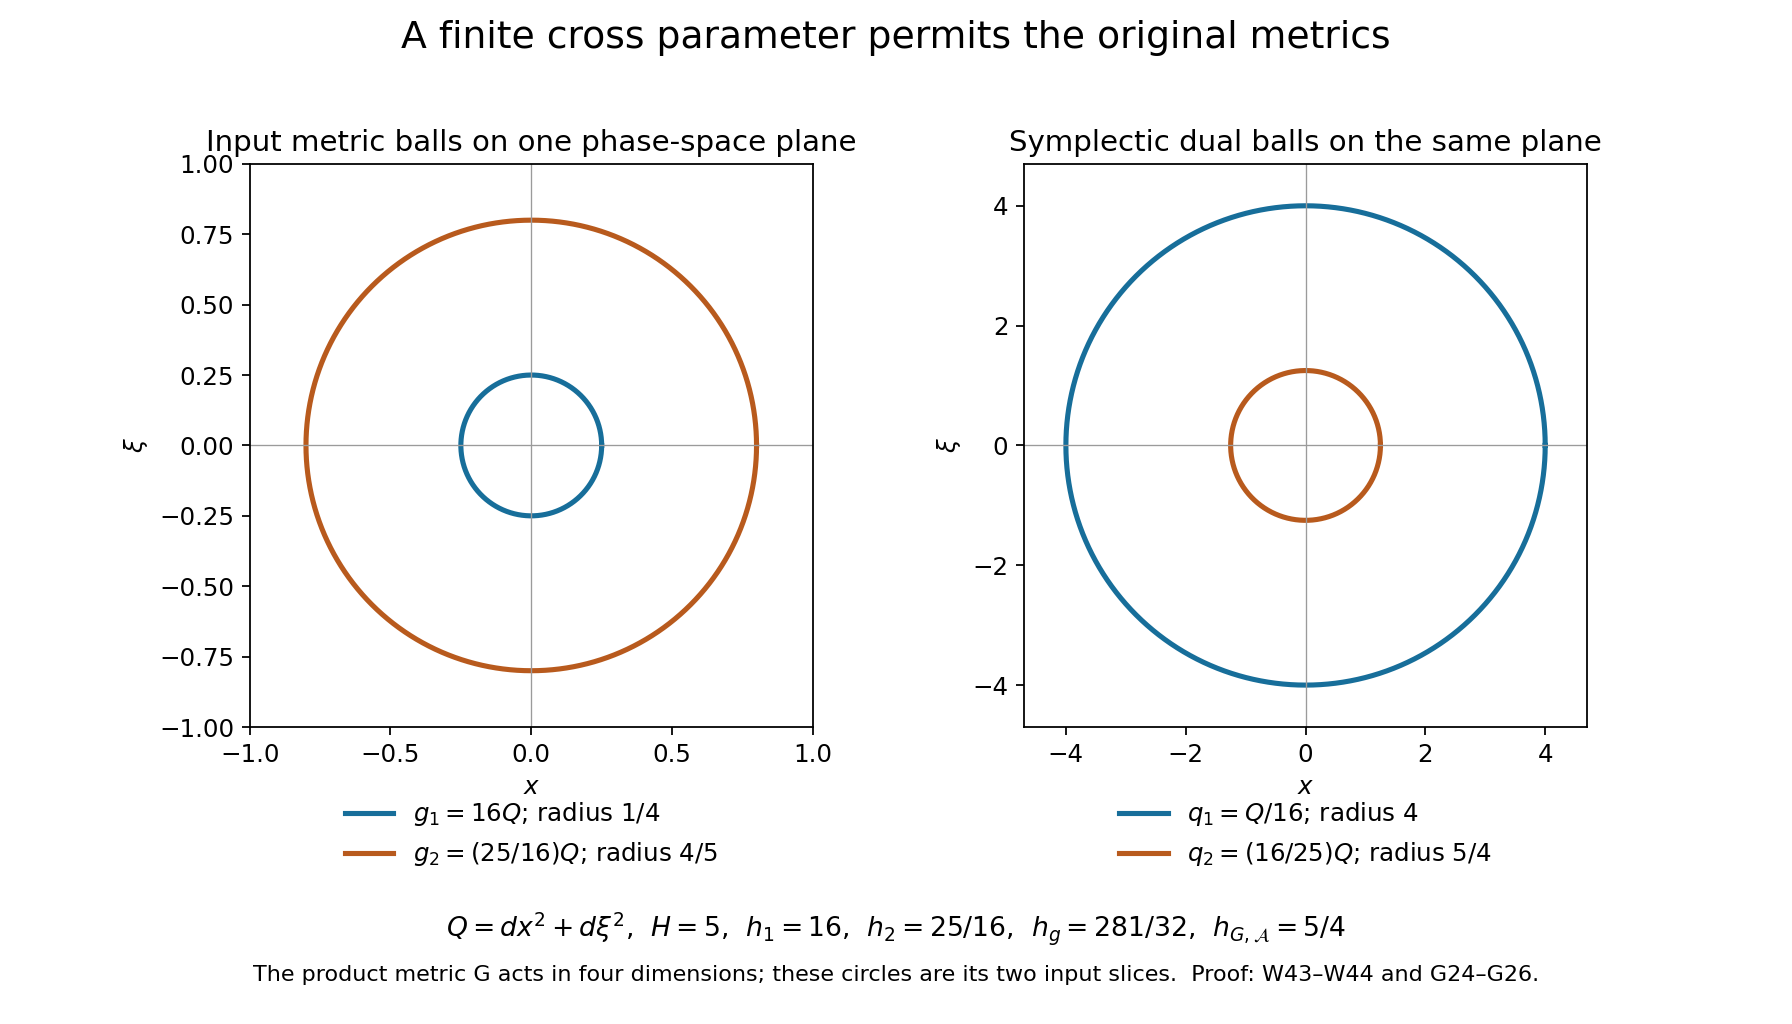
\includegraphics[keepaspectratio]{../figures/weyl-bounded-cross-parameter.png}}
\caption{The original metric balls for the bounded cross-parameter
example}
\end{figure}

\textbf{Polynomial termination.} If either factor in the theorem is a
polynomial of total degree less than \(N\), then \(R_N(a,b)=0\). Here is
a justification that also covers a noncompact second factor. For
compactly supported smooth \(u\) on the product space, Taylor's integral
formula gives, for \(N\geq1\), \[
T_{\mathcal A}u-\sum_{j<N}(i\mathcal A(D))^ju/j!
=\frac{i^N}{(N-1)!}\int_0^1(1-t)^{N-1}
T_{t\mathcal A}\big(\mathcal A(D)^Nu\big)\,dt.
\tag{W35}
\] This identity extends to the bounded-symbol restriction on the
diagonal. To see the needed continuity, expand \(\mathcal A(D)^N\) into
its finitely many constant-coefficient directional derivatives. For a
term \(\partial_{V_1}\cdots\partial_{V_{2N}}u\), use the weight
\(M_V(Z)=M(Z)\prod_\ell G_Z(V_\ell)^{1/2}\), as in Theorem 7.1 of
\href{gauss-transform-estimates.pdf}{Quadratic Fourier multipliers at a
moving scale}. It is locally continuous and phase-temperate along the
diagonal by the product-metric comparisons already proved. The
corresponding Gauss evaluation estimate is uniform for \(0< t\leq1\):
its dual distance is \(t^{-2}G^{\mathcal A}\), so the same temperateness
constants work and its uncertainty bound is no larger. At \(t=0\), use
ordinary evaluation. These estimates give a common integrable bound in
(W35). Bounded compactly supported approximation, weak continuity for
each \(t\), and dominated convergence extend (W35) term by term. This
argument needs only finitely many modified weights.

Every term of \(\mathcal A(D_X,D_Y)^N(a\otimes b)\) differentiates each
factor exactly \(N\) times. Thus it is identically zero when either
polynomial has degree less than \(N\). The right side of (W35) vanishes,
proving termination. The assertion concerns a polynomial that belongs to
the specified input symbol space; it does not assert membership for
every polynomial and every weight.

\textbf{One metric and scalar parity.} Taking \(g_1=g_2=g\), \(H=h_g\),
gives the full one-metric theorem under \(g\leq g^\sigma\). For scalar
symbols, interchanging the two arguments changes \(\mathcal A\) to
\(-\mathcal A\). Hence \(C_j(b,a)=(-1)^jC_j(a,b)\). Apply (W32) with
\(N=3\) to the difference and with \(N=2\) to the sum. Using (W29) gives
\[
a\#b-b\#a-\{a,b\}/i\in S(h_g^3m_1m_2,g),
\qquad
a\#b+b\#a-2ab\in S(h_g^2m_1m_2,g).
\tag{W36}
\] The even/odd cancellation uses commutativity of scalar
multiplication. Applying it unchanged to matrix symbols would be
incorrect.

Equations (W31)--(W36) construct a symbol product and its estimates.
Equation \((a\#b)^w=a^wb^w\) has been proved here for Schwartz symbols.
For arbitrary metric symbols the composition on the right needs a common
operator domain and continuity theorem; that is a separate general
operator-calculus theorem. It is not inferred from two maps
\(\mathcal S\to\mathcal S'\), whose composite need not be defined.

\subsection{8. Classical parameter ranges and quantization
changes}\label{classical-parameter-ranges-and-quantization-changes}

Consider, for real \(\mu\), \[
g_{(x,\xi)}(y,\eta)=\langle\xi\rangle^{2\delta}|y|^2+
\langle\xi\rangle^{-2\rho}|\eta|^2,
\qquad m(x,\xi)=\langle\xi\rangle^\mu,
\quad 0\leq\delta\leq\rho\leq1,\quad\delta<1.
\tag{W37}
\] \href{metric-localization.pdf\#section*.29}{An anisotropic
model} proves slow variation and local weight continuity. Direct
quadratic inversion gives \[
g_{(x,\xi)}^\sigma(y,\eta)
=\langle\xi\rangle^{2\rho}|y|^2+
\langle\xi\rangle^{-2\delta}|\eta|^2,
\qquad h_g=\langle\xi\rangle^{\delta-\rho}\leq1.
\tag{W38}
\]

We verify the global condition, including the endpoint. Let
\(r=\langle\eta\rangle\), \(s=\langle\xi\rangle\), \(d=|\eta-\xi|\). It
suffices to bound \[
(r/s)^{2\delta}+(s/r)^{2\rho}
\leq C(1+d^2r^{-2\delta})^L.
\tag{W39}
\] If \(r/2\leq s\leq2r\), the left side is bounded. If \(r>2s\), the
Lipschitz property of \(\langle\cdot\rangle\) gives \(d\geq r-s>r/2\),
so the base on the right is at least a constant times
\(r^{2(1-\delta)}\). Since \(s\geq1\), an exponent
\(L\geq\delta/(1-\delta)\) controls the first ratio; the second is at
most one. If \(s>2r\), then \(d>s/2\), and
\(d^2r^{-2\delta}\geq(s/r)^2/4\) because \(r\geq1\) and \(\delta\leq1\).
Now \(L\geq\rho\) works. This proves (W39) and metric temperateness. The
same three cases control \((r/s)^\mu\): in the second case take
\(2L(1-\delta)\geq\max(\mu,0)\), and in the third take
\(2L\geq\max(-\mu,0)\). Thus every indicated real-order weight is
temperate.

The class \(S(m,g)\) is exactly \(S^\mu_{\rho,\delta}\). The product
theorem therefore has remainder order \(\mu_1+\mu_2-N(\rho-\delta)\).
When \(\delta=\rho<1\), it remains a continuous closure and
finite-remainder theorem, but the order does not decrease with \(N\).
This is not an asymptotic expansion in decreasing orders at that
endpoint. At \((\rho,\delta)=(1,1)\), (W39) fails: take \(s=1\),
\(r\to\infty\); its right-hand base stays bounded while the first ratio
grows. The present argument therefore excludes type \((1,1)\).

For completeness the same metric calculation proves the full symbol
change between the quantizations (W19). For fixed real \(\tau,s\), set
\[
b=\exp\big(i(\tau-s)\langle D_x,D_\xi\rangle\big)a.
\tag{W40}
\] Then \(\operatorname{Op}_s(b)=\operatorname{Op}_\tau(a)\) as
distributional kernels. One can verify the sign on a plane wave: in the
kernel coordinates for \(s\), the old base point is \(z+(s-\tau)t\).
Partial Fourier inversion sets \(t=-q\), giving the factor
\(e^{i(\tau-s)p\cdot q}\), exactly the multiplier in (W40). Fourier
transformation and invertible linear coordinate changes extend this
identity to all tempered distributions.

For the auxiliary phase \(2\langle D_x,D_\xi\rangle\), the phase-dual
metric is (W38). For the actual phase in (W40), its Gauss parameter is
\(|\tau-s|h_g/2\). We retain the original \(g\) and apply the
finite-bound form (G24)--(G26) of
\href{gauss-transform-estimates.pdf\#section*.46}{Theorem
8.1}. Here is its exact receiving calculation, including every
quantization-parameter factor.

Put \(c=\tau-s\), and first suppose \(n\geq1\) and \(c\ne0\). On the
original \(2n\)-dimensional phase space, the quadratic phase and its
associated symmetric map are \[
 A_c(p,q)=c\,p\cdot q,\qquad
 B_c=\frac c2
 \begin{pmatrix}0&I_n\\ I_n&0\end{pmatrix},\qquad
 g_X(B_c(p,q))=\frac{c^2}{4}
 \big(\langle\xi\rangle^{2\delta}|q|^2+
      \langle\xi\rangle^{-2\rho}|p|^2\big).
 \tag{WQ1}
\] The map is invertible. The supremum definition (G1), or the dual of
the displayed positive quadratic form, gives on every original direction
\(T=(y,\eta)\) \[
 g_X^{A_c}(y,\eta)=\frac4{c^2}
 \big(\langle\xi\rangle^{2\rho}|y|^2+
      \langle\xi\rangle^{-2\delta}|\eta|^2\big)
 =\frac4{c^2}g_X^\sigma(y,\eta),\qquad
 h_{g,A_c}(X)=\frac{|c|}{2}\langle\xi\rangle^{\delta-\rho}
 \leq h_*=\frac{|c|}{2}.
 \tag{WQ2}
\] Indeed, the ratio of the coefficient of each component in the
original metric to its coefficient in the displayed phase-dual metric is
exactly \(c^2\langle\xi\rangle^{2(\delta-\rho)}/4\). Thus the supremum
in (G3) gives precisely (WQ2), with no lost component or exceptional
nonzero direction.

The original temperateness inequalities use the whole symplectic-dual
distance. Their comparison with the actual phase-dual distance is \[
 1+g_Y^\sigma(X-Y)
 =1+\frac{c^2}{4}g_Y^{A_c}(X-Y)
 \leq \max(1,c^2/4)\big(1+g_Y^{A_c}(X-Y)\big).
 \tag{WQ3}
\] Consequently a metric inequality with exponent \(L\) retains its
original constant multiplied by \(\max(1,c^2/4)^L\); a weight inequality
retains the corresponding factor with its own original exponent. Slow
variation and local weight continuity use the original metric and are
unchanged. The observation space is the entire original phase space.
These statements verify all hypotheses of (G24) and (G13), including the
actual structural constants. In the counting step (G25), the retained
dimension is \(2n\), so the additional finite-bound factor is
\((1+|c|/2)^{2n}\). This is one factor entering the theorem's constant;
it is not a claim that this factor alone accounts for every dependence
on \(c\).

For every integer \(N\geq0\) and every derivative order \(l\), (G26) now
proves \[
 \begin{split}
 |\partial_{T_1}\cdots\partial_{T_l}R_Na(X)|
 &\leq C_{N,l,|c|/2}\,
       \langle\xi\rangle^\mu
       \left(\frac{|c|}{2}
                  \langle\xi\rangle^{\delta-\rho}\right)^N\\
 &\quad{}\times
       \prod_{j=1}^l
       \left(\langle\xi\rangle^{2\delta}|y_j|^2+
             \langle\xi\rangle^{-2\rho}|\eta_j|^2\right)^{1/2}
       p_{\leq J_{N,l}}(a;m,g),\\
 R_Na&=T_{A_c}a-\sum_{j<N}\frac{(iA_c(D))^j}{j!}a,
 \qquad T_j=(y_j,\eta_j).
 \end{split}
 \tag{WQ4}
\] The constants include the actual metric and weight constants just
computed. In particular, the full target weight is
\((|c|/2)^N\langle\xi\rangle^{\mu-N(\rho-\delta)}\). For this fixed
nonzero parameter its constant factor yields the stated class inclusion,
while (WQ4) keeps the factor in the estimate.

The original Taylor terms agree exactly with those in the quantization
formula: \[
 \begin{split}
 \sum_{j<N}\frac{(iA_c(D))^j}{j!}a
 &=\sum_{j<N}\frac{i^jc^j}{j!}
       \sum_{|\alpha|=j}\frac{j!}{\alpha!}
                     D_x^\alpha D_\xi^\alpha a\\
 &=\sum_{j<N}\sum_{|\alpha|=j}
       \frac{i^j(-i)^jc^j}{\alpha!}
                     \partial_\xi^\alpha D_x^\alpha a
 =\sum_{|\alpha|<N}\frac{c^{|\alpha|}}{\alpha!}
                     \partial_\xi^\alpha D_x^\alpha a.
 \end{split}
 \tag{WQ5}
\] Here all coordinate derivatives commute, \(D_\xi=-i\partial_\xi\),
and \(i^j(-i)^j=1\). The finite sum is empty for \(N=0\). If \(c=0\),
the multiplier is the identity: its remainder is zero for \(N\geq1\),
and its zeroth remainder is the identity. The term of order zero has
coefficient one, so no undefined zero power is used. If \(n=0\), the
phase space has one point, the operator is again the identity for every
\(c\), and the same remainder statements hold directly. No positive
phase parameter is assigned to that zero-dimensional identity case. This
proves, on the original metric, \[
b-\sum_{|\alpha|<N}
\frac{(\tau-s)^{|\alpha|}}{\alpha!}
\partial_\xi^\alpha D_x^\alpha a
\ \in\ S^{\mu-N(\rho-\delta)}_{\rho,\delta}.
\tag{W41}
\] The map and every remainder are continuous with finite
source-seminorm control, and weakly continuous on bounded symbol sets.
The zero phase is the identity and is handled directly. Constants may
depend on \(\tau-s\); no uniformity over unbounded quantization
parameters is claimed.

These classical symbols are tempered, since all coordinate derivatives
have polynomial growth in \(\xi\), uniformly in \(x\). Bounded symbol
approximants that converge locally smoothly converge also in
\(\mathcal S'\): their common polynomial growth bound and the rapid
decay of a Schwartz test function give dominated convergence. Thus the
Gauss extension used in (W40) agrees with its distributional Fourier
multiplier, since both are limits of the same compactly supported
approximants, and the Gauss limit is locally smooth on the whole phase
space. Their left quantizations map \(\mathcal S\) continuously into
\(\mathcal S\): write the output as
\((2\pi)^{-n}\int e^{ix\cdot\xi}a(x,\xi)\widehat u(\xi)\,d\xi\). Any
output derivative introduces finitely many polynomial factors and symbol
derivatives. To multiply by \(x^\alpha\), integrate by parts
\(|\alpha|\) times in \(\xi\). Each term is bounded uniformly in \(x\)
by finitely many Schwartz seminorms of \(u\), after choosing a
sufficiently integrable negative power of \(\langle\xi\rangle\). This
proves all output Schwartz seminorms. The other quantizations have the
same mapping property by (W40).

In particular, the adjoint of a left quantization has left symbol
\(\exp(i\langle D_x,D_\xi\rangle)\overline a\), which is in the same
class by (W40). Transposition of its continuous Schwartz action extends
the original operator continuously to \(\mathcal S'\). This classical
statement is proved using (W37); it does not close the separate
arbitrary-metric operator dependency.

\subsubsection{8.1. The full parameter range for the same original
metric}\label{the-full-parameter-range-for-the-same-original-metric}

The nonnegative range in (W37) remains its original statement. The
following separate extension proves that the same metric, weight, symbol
class, product and quantization formulas work for \[
 n\geq1,\qquad \delta\leq\rho\leq1,\qquad\delta<1,\qquad
 \mu\in\mathbb R.
 \tag{WX1}
\] In particular, negative values of either parameter are allowed
subject to these inequalities. This is a strengthening of the local
statement, with no novelty claim and no claim about the separate
arbitrary-metric operator entry.

\textbf{Slow variation and local weight continuity.} Use the original
metric of (W37). If \(X=(x,\xi)\), \(Y=X+(y,\eta)\),
\(s=\langle\xi\rangle\), and \(g_X(Y-X)\leq r_*^2\) with \(0<r_*<1/2\),
then \[
 |\eta|\leq r_*s^\rho\leq r_*s,\qquad
 (1-r_*)s\leq\langle\xi+\eta\rangle\leq(1+r_*)s.
 \tag{WX2}
\] The first bound uses exactly \(\rho\leq1\) and \(s\geq1\); the second
uses the Lipschitz bound for the original bracket function. For any
fixed real exponent \(v\), put \[
 a_v=\min\{(1-r_*)^v,(1+r_*)^v\},\qquad
 b_v=\max\{(1-r_*)^v,(1+r_*)^v\}.
 \tag{WX3}
\] Then \(0<a_v\leq(\langle\xi+\eta\rangle/s)^v\leq b_v<\infty\).
Applying this to \(v=2\delta,-2\rho,\mu\) compares both separate
coefficients of the original metric and the original weight. For every
direction \(T\), \[
 \min(a_{2\delta},a_{-2\rho})g_X(T)
 \leq g_Y(T)\leq
 \max(b_{2\delta},b_{-2\rho})g_X(T),\qquad
 a_\mu m(X)\leq m(Y)\leq b_\mu m(X).
 \tag{WX4}
\] This proves the two local hypotheses, including negative exponents;
it is the exact arbitrary-real-exponent calculation in
\href{metric-localization.pdf\#section*.29}{the anisotropic
model}.

\textbf{Global temperateness.} For arbitrary \(X=(x,\xi)\) and
\(Y=(y,\eta)\), retain \(r=\langle\eta\rangle\),
\(s=\langle\xi\rangle\), \(d=|\eta-\xi|\), and define \[
 B=1+d^2r^{-2\delta}
 \leq 1+g_Y^\sigma(X-Y)
 =1+r^{2\rho}|x-y|^2+r^{-2\delta}|\xi-\eta|^2.
 \tag{WX5}
\] Choose a nonnegative integer \[
 L\geq\max\left\{0,\frac{\delta}{1-\delta},
                    \frac{-\rho}{1-\delta},-\delta,\rho\right\},
 \qquad
 C=\max\{2^{2|\delta|}+2^{2|\rho|},\,2\,4^L\}.
 \tag{WX6}
\] We prove the full left side of (W39) is at most \(CB^L\). If
\(r/2\leq s\leq2r\), the two summands are at most \(2^{2|\delta|}\) and
\(2^{2|\rho|}\). If \(r>2s\), put \(a=\max(\delta,-\rho,0)\). Since
\(r/s\leq r\) and \(s\geq1\), each summand is at most \(r^{2a}\). The
Lipschitz bound gives \(d\geq r-s>r/2\), hence \[
 B\geq\frac14r^{2(1-\delta)},\qquad
 (r/s)^{2\delta}+(s/r)^{2\rho}
 \leq2r^{2a}\leq2\,4^LB^L.
 \tag{WX7}
\] The last inequality uses \(L(1-\delta)\geq a\). If \(s>2r\), put
\(b=\max(-\delta,\rho,0)\). Each summand is at most \((s/r)^{2b}\),
whereas \[
 B\geq d^2r^{-2\delta}>
       \frac14(s/r)^2r^{2(1-\delta)}
 \geq\frac14(s/r)^2,\qquad
 (r/s)^{2\delta}+(s/r)^{2\rho}
 \leq2(s/r)^{2b}\leq2\,4^LB^L.
 \tag{WX8}
\] Here \(r\geq1\), \(1-\delta>0\), and \(L\geq b\). All three cases
prove (W39) with the explicit constants (WX6). For each original
direction, the ratio of the spatial coefficients is \((r/s)^{2\delta}\),
and the ratio of the frequency coefficients is \((s/r)^{2\rho}\). Their
sum controls the whole quadratic-form comparison. Equation (WX5) gives
its required full dual-distance bound. Interchanging \(X,Y\) proves the
other ordered metric comparison; no spatial-distance term is removed
from that comparison.

For the original weight ratio choose a nonnegative integer and constant
\[
 L_\mu\geq\max\left\{0,
             \frac{\max(\mu,0)}{2(1-\delta)},
             \frac{\max(-\mu,0)}2\right\},\qquad
 C_\mu=\max\{2^{|\mu|},4^{L_\mu}\}.
 \tag{WX9}
\] In the comparable case \((r/s)^\mu\leq2^{|\mu|}\). If \(r>2s\), this
ratio is at most \(r^{\max(\mu,0)}\), and (WX7) bounds it by
\(4^{L_\mu}B^{L_\mu}\). If \(s>2r\), the ratio is at most
\((s/r)^{\max(-\mu,0)}\), and (WX8) gives the same bound. Thus the full
original weight is temperate in each ordered direction.

\textbf{Uncertainty and the actual receiving formulas.} Direct
comparison of each coefficient in (W37) and (W38) gives \[
 g_X(T)=\langle\xi\rangle^{2(\delta-\rho)}g_X^\sigma(T)
 \leq g_X^\sigma(T),\qquad
 h_g(X)=\langle\xi\rangle^{\delta-\rho}.
 \tag{WX10}
\] To identify the symbol space without changing the metric, apply its
directional bounds to each original coordinate vector. A spatial vector
has length \(s^\delta\), and a frequency vector has length
\(s^{-\rho}\). This gives \[
 |\partial_x^\beta\partial_\xi^\alpha a(x,\xi)|
 \leq C_{\alpha,\beta}
       \langle\xi\rangle^{\mu+\delta|\beta|-\rho|\alpha|}.
 \tag{WX11}
\] Conversely, expand any \(k\) original directional derivatives into
the \((2n)^k\) coordinate choices, retaining each coefficient. For every
\(T=(y,\eta)\), \[
 |y_j|\leq s^{-\delta}g_X(T)^{1/2},\qquad
 |\eta_j|\leq s^\rho g_X(T)^{1/2}.
 \tag{WX12}
\] Each coordinate term in (WX11) therefore costs at most its constant
times \(s^\mu\prod_jg_X(T_j)^{1/2}\); the powers from its directions
cancel the corresponding derivative powers exactly. The finite sum
proves the reverse bound with finite coordinate-seminorm control. This
proves the exact class identification in both directions.

The already proved one-metric product theorem applies with
\(g_1=g_2=g\); its actual parameter is \(H=h_g\), and its full remainder
weight is \(m_1m_2h_g^N\). It gives the original coefficient formulas
and remainder order \(\mu_1+\mu_2-N(\rho-\delta)\), with every factor
retained in its estimates. The calculation (WQ1)--(WQ5) applies verbatim
to (WX1): it keeps the factor \((|c|/2)^N\), every phase-dependent
structural constant, and the same zero cases, so it proves (W40)--(W41)
throughout this range. The Schwartz and tempered-distribution arguments
following (W41) also apply: for each fixed derivative, the exponent in
(WX11) is a finite real number, hence it is bounded by an integer
polynomial growth exponent; Schwartz decay supplies each required
integrable majorant. This proves their stated continuity and kernel
identities for negative parameters too. At \(\delta=\rho<1\), the
remainder order is unchanged; an order improvement is not asserted.
\textbf{Editorial completion of the classical operator product.}
Throughout (WX1), the symbol product also gives the exact composite on
the original Schwartz space and its tempered dual. We prove the operator
convergence needed for this statement, rather than composing two
arbitrary Schwartz-to-distribution maps.

Let \(q_{\nu,\lambda}(a)\) denote the supremum of the absolute value of
\(\partial_\xi^\nu\partial_x^\lambda a\) divided by its full weight
\(\langle\xi\rangle^{\mu+\delta|\lambda|-\rho|\nu|}\) in (WX11). For
\(u\in\mathcal S\), retain the original left formula and Fourier
transform. Differentiation, followed by integration by parts in \(\xi\),
gives every original output seminorm through the identity \[
 \begin{aligned}
 x^\alpha\partial_x^\beta\operatorname{Op}_0(a)u(x)
 &=(2\pi)^{-n}i^{|\alpha|}
   \sum_{\lambda\leq\beta}\binom\beta\lambda
   \sum_{\kappa+\nu+\omega=\alpha}
         \frac{\alpha!}{\kappa!\nu!\omega!}\\
 &\quad\times\int e^{ix\cdot\xi}
       P_{\beta-\lambda,\kappa}(\xi)
       (\partial_\xi^\nu\partial_x^\lambda a)(x,\xi)
       (\partial_\xi^\omega\widehat u)(\xi)\,d\xi,\\
 P_{v,\kappa}(\xi)&=
 \begin{cases}
 i^{|v|}\dfrac{v!}{(v-\kappa)!}\xi^{v-\kappa},&\kappa\leq v,\\
 0,&\kappa\not\leq v.
 \end{cases}
 \end{aligned}
 \tag{WO1}
\] The polynomial derivative, all zero terms, all multinomial terms, the
original inverse factor and the integration-by-parts sign
\((-1)^{|\alpha|}i^{-|\alpha|}=i^{|\alpha|}\) remain. The integrals and
integrations by parts are justified by Schwartz decay, using the same
bounds now displayed explicitly. For a nonzero polynomial term set \[
 E_{\lambda,\kappa,\nu}=
    |\beta-\lambda-\kappa|+\mu+\delta|\lambda|-\rho|\nu|,
 \quad
 U_{M,\omega}(u)=\sup_\xi\langle\xi\rangle^M
                          |\partial_\xi^\omega\widehat u(\xi)|.
 \tag{WO2}
\] Choose an integer \(M>n+\max E_{\lambda,\kappa,\nu}\) over this
finite set. The full bound for the original output seminorm is \[
 \begin{aligned}
 p_{\alpha,\beta}(\operatorname{Op}_0(a)u)
 &\leq(2\pi)^{-n}
 \sum_{\lambda\leq\beta}\binom\beta\lambda
 \sum_{\substack{\kappa+\nu+\omega=\alpha\\\kappa\leq\beta-\lambda}}
 \frac{\alpha!(\beta-\lambda)!}
      {\kappa!\nu!\omega!(\beta-\lambda-\kappa)!}\\
 &\quad\times q_{\nu,\lambda}(a)U_{M,\omega}(u)
             \int\langle\xi\rangle^{E_{\lambda,\kappa,\nu}-M}\,d\xi.
 \end{aligned}
 \tag{WO3}
\] Each integral is finite by the full dyadic volume estimate with
exponent less than \(-n\). Each \(U_{M,\omega}\) is a continuous
seminorm of the original Schwartz input, by the Fourier prerequisite and
the complete monomial comparison (WK3). Therefore (WO3) proves the
actual continuous map
\(\operatorname{Op}_0(a):\mathcal S\to\mathcal S\), with finite
symbol-seminorm control, for every real parameter in (WX1).

We need more than this bound. If \(a_j\to a\) locally smoothly in a
bounded set of the same original symbol class, then
\(\operatorname{Op}_0(a_j)\to\operatorname{Op}_0(a)\) uniformly on each
bounded Schwartz input set, in every original Schwartz output seminorm.
Here are both tails. Write \(v_j=\operatorname{Op}_0(a_j-a)u\). For
\(|x|>R\), some coordinate has \(|x_i|>R/\sqrt n\), so \[
 |x^\alpha\partial^\beta v_j(x)|
 \leq\frac{\sqrt n}{R}
             \max_i p_{\alpha+e_i,\beta}(v_j).
 \tag{WO4}
\] These higher seminorms are uniformly bounded by (WO3), for the
bounded symbol differences and bounded inputs. On \(|x|\leq R\), split
every original integral (WO1) into \(|\xi|\leq S\) and its complement.
The bounded input set has uniformly bounded \(U_{M,\omega}\); choose
\(M\) one larger than required in (WO3). The same complete integrable
majorants then give frequency tails tending to zero uniformly in
\(j,u,x\). On the finite \((x,\xi)\) box, every symbol derivative in the
finite sums tends uniformly to zero, and the test derivatives are
uniformly bounded, so the remaining integrals tend uniformly to zero.
First choose \(R,S\), then \(j\). Equations (WO1)--(WO4) prove the
asserted convergence without omitting spatial or frequency tails.

For a fixed real quantization parameter \(\tau\), (W40) with \(s=0\)
expresses \(\operatorname{Op}_\tau(a)\) as
\(\operatorname{Op}_0(T_{A_\tau}a)\). The complete calculation
(WQ1)--(WQ5) proves finite-seminorm continuity and bounded-set local
smooth continuity in the same original symbol class, keeping every
\(\tau\) factor and its zero case. Thus all the continuity and
convergence assertions above hold for the original Weyl operator too.

Now let \(a\in S^{\mu_1}_{\rho,\delta}\),
\(b\in S^{\mu_2}_{\rho,\delta}\) in (WX1). Choose the original bounded
compactly supported approximants \(a_j,b_j\) from the localization
prerequisite. They converge locally smoothly in their respective bounded
classes, and the product theorem gives \(c_j=a_j\#b_j\to c=a\#b\)
locally smoothly in a bounded subset of the full class of order
\(\mu_1+\mu_2\). The Schwartz-symbol identity (W27) holds for each pair.
Put \(A_j=a_j^w\), \(B_j=b_j^w\), \(A=a^w\), \(B=b^w\). For each
original \(u\in\mathcal S\), the sequence \(B_ju\) converges to \(Bu\)
in \(\mathcal S\) and hence is bounded there. Consequently \[
 A_jB_ju-ABu=(A_j-A)B_ju+A(B_ju-Bu)\longrightarrow0
                     \quad\text{in }\mathcal S.
 \tag{WO5}
\] The first term uses the just-proved uniform convergence on bounded
input sets; the second uses actual Schwartz continuity of \(A\). Also
\(c_j^wu\to c^wu\) in \(\mathcal S\). Passing to the limit proves the
exact equality \[
 (a\#b)^w=a^wb^w:\mathcal S\longrightarrow\mathcal S.
 \tag{WO6}
\] All domains are the entire original Schwartz space. This closes the
composition for the classical parameter range, without asserting an
unspecified \(L^2\) closure or a product for arbitrary metric symbols.

For completeness these maps extend continuously to the original strong
tempered dual, and (WO6) holds there too. Write \(C\) for complex
conjugation on tests and \(A^t=C(\overline a)^wC\). Equation (W21)
proves the exact bilinear transpose identity on every Schwartz pair;
both conjugations and the middle Schwartz map are continuous, and their
composite is linear. Define \(\widetilde A T\) by
\((\widetilde A T)(v)=T(A^tv)\). For any bounded test set \(F\), the
image \(A^tF\) is bounded, so its full strong-dual seminorm is exactly
\(T_F(\widetilde A T)=T_{A^tF}(T)\). This proves strong continuity. On
distributions represented by Schwartz functions it is the original
\(A\), by the transpose identity. The transpose of the composite in
(WO6) is \(B^tA^t\), with its full order retained, since evaluation on
every pair gives this identity. Therefore \[
 \widetilde{(a\#b)^w}=\widetilde{a^w}\,\widetilde{b^w}
                    :\mathcal S'\longrightarrow\mathcal S'.
 \tag{WO7}
\] The kernel bijection (W20), already proved by (WK1)--(WK24), is
injective. Associativity of the actual continuous Schwartz composites
and (WO6) thus prove \((a\#b)\#c=a\#(b\#c)\) for three classical symbols
in this same parameter range, in the full class of order
\(\mu_1+\mu_2+\mu_3\).

The same statements also give exact finite matrix receiving maps, with
no scalar parity assumption. For matrices \(a\) of size \(p\times q\)
and \(b\) of size \(q\times r\), with each entry in its stated scalar
input class, define \[
 (a\#b)_{ij}=\sum_{v=1}^q a_{iv}\#b_{vj},\quad
 C_j(a,b)_{i\ell}=\sum_{v=1}^q C_j(a_{iv},b_{v\ell}),\quad
 R_N(a,b)_{i\ell}=\sum_{v=1}^q R_N(a_{iv},b_{v\ell}).
 \tag{WO8}
\] Every intermediate index and its order remain. The scalar bounds
(W33), or (WG4) with unbounded \(H\), apply to every summand; the output
seminorm is at most their complete finite sum. This proves the
corresponding distinct-metric and classical matrix symbol maps, with the
same explicit target weights. In the classical case (WO6) gives the
exact composite \(\mathcal S(V)^r\to\mathcal S(V)^p\), and (WO7) gives
its tempered-dual composite. Finite sums of the component proofs give
continuity and associativity on their stated domains. Interchanging
square matrices does not supply the scalar cancellations in (W36); no
matrix summand has been commuted.

\textbf{Why these three hypotheses are exact for this metric argument.}
They cannot be dropped from the simultaneous slow-variation, uncertainty
and temperateness hypotheses when \(n\geq1\). If \(\rho>1\), take
\(X_t=(0,te_1)\), \(Y=(0,0)\) and \(T=(0,e_1)\). Then \[
 g_{X_t}(Y-X_t)=t^2(1+t^2)^{-\rho}\longrightarrow0,\qquad
 \frac{g_Y(T)}{g_{X_t}(T)}=(1+t^2)^\rho\longrightarrow\infty.
 \tag{WX13}
\] This violates slow variation for every proposed fixed local radius
and comparison constant. If \(\delta>\rho\), the exact coefficient ratio
in (WX10) tends to infinity as \(|\xi|\to\infty\), so the required
uncertainty comparison fails. Finally, under \(\delta\leq\rho\leq1\),
the remaining possibility \(\delta\geq1\) is \(\delta=\rho=1\). Take
\(X=(0,0)\), \(Y=(0,\eta)\) and the spatial direction \(T=(e_1,0)\).
Then \[
 \frac{g_Y(T)}{g_X(T)}=\langle\eta\rangle^2,\qquad
 g_Y^\sigma(X-Y)=\frac{|\eta|^2}{\langle\eta\rangle^2}<1.
 \tag{WX14}
\] No fixed constant and finite exponent can give the required ordered
temperateness inequality. These are exact failures of those hypotheses,
not assertions that every alternative calculus is impossible outside
this range. For \(n=0\), all spaces here have one point, every
positive-order coordinate derivative is absent, every Fourier factor is
\((2\pi)^0=1\), and the scalar product and identity quantization
formulas hold for all parameters. The remainders are zero for \(N\geq1\)
and the identity for \(N=0\), treated directly without a positive phase
weight. \(\square\) \textbf{Editorial zero-dimensional receiving maps.} In the
sole-point case the zeroth product remainder is the bilinear map
\(R_0(a,b)=ab\), while the zeroth quantization-change remainder is the
linear identity \(R_0a=a\). Their positive-order remainders are both
zero. These are distinct original maps; the word identity in the
preceding endpoint paragraph refers to quantization change. The scalar
product, the actual coefficient-one Fourier factor, and every
empty-coordinate convention remain.

\subsection{9. An example beyond one-metric
uncertainty}\label{an-example-beyond-one-metric-uncertainty}

Take a standard symplectic Euclidean form \(Q\) with \(Q^\sigma=Q\), and
choose constants \(L>1\), \(0<\varepsilon\leq1\). Let \[
g_1=LQ,\qquad g_2=\varepsilon^2L^{-1}Q,\qquad m_1=m_2=1.
\tag{W42}
\] All local and cross comparisons are constant. The duals are
\(L^{-1}Q\) and \(L\varepsilon^{-2}Q\), so \(H=\varepsilon\). But
\(h_1=L\), and \(h_g=(L+\varepsilon^2/L)/2\), which exceeds one when
\(L\) is large. Theorem (W31) still applies, with the \(\varepsilon^N\)
remainder bound. Thus replacing its hypotheses by uncertainty of the
mean would discard actual valid cases. Letting \(L\) grow also separates
\(H\) from \(h_g\) by an arbitrarily large ratio.

As a normalization check in one dimension, (W23) gives
\(x\#\xi=x\xi+i/2\) and \(\xi\#x=x\xi-i/2\). Their difference is \(i\),
agreeing with \([x,D]=i\). Since either factor has degree one, every
remainder with \(N\geq2\) vanishes exactly.

\subsection{10. Exercises and solutions}\label{exercises-and-solutions}

\textbf{Problem 1.} On \(\mathbb R^2\), take \(g_1=9Q\), \(g_2=Q/36\).
Compute \(H,h_1,h_2,h_g\). Which theorem applies to their product?

\textbf{Solution.} Their duals are \(Q/9\) and \(36Q\). Thus
\(H^2=9/36=1/4\), \(H=1/2\), while \(h_1=9\), \(h_2=1/36\). The mean is
\((325/72)Q\), so \(h_g=325/72\). The distinct-metric theorem applies
with remainder weight \(2^{-N}\); its one-metric specialization applied
to the mean does not meet its uncertainty hypothesis. Each chosen symbol
must, of course, have the derivative bounds in its own stated metric.

\textbf{Problem 2.} Prove the sharp scalar version of (W5) for
\(g_1(t)=a t^2\), \(g_2(t)=b t^2\), \(a,b>0\), using ordinary duality in
place of \(\sigma\).

\textbf{Solution.} Minimize \(2((t-z)^2/a+z^2/b)\). Differentiation
gives \(z=bt/(a+b)\). Substitution gives \(2t^2/(a+b)\), which is the
ordinary dual of \((a+b)t^2/2\). The missing factor two would give the
wrong dual even when \(a=b=1\).

\textbf{Problem 3.} Let \(a(x,\xi)=x^2\), \(b(x,\xi)=\xi^2\) in one
dimension, with polynomial weights that contain them. Compute the exact
Weyl product and its operator.

\textbf{Solution.} The zeroth term is \(x^2\xi^2\); the first is
\(\{x^2,\xi^2\}/(2i)=2ix\xi\). The only second-order term differentiates
twice in \(x\) in the first factor and twice in \(\xi\) in the second;
its coefficient is \((i/2)^2/2!=-1/8\), so its value is \(-1/2\). All
later terms vanish. Therefore \(x^2\#\xi^2=x^2\xi^2+2ix\xi-1/2\). Its
Weyl operator equals \(x^2D^2\): apply (W23) twice to multiplication by
\(x\), starting with \(\xi^2\). This polynomial calculation defines the
composite on \(\mathcal S\) directly, so it does not require the
unresolved general operator theorem.

\textbf{Problem 4.} For \(\rho=\delta=2/3\), what does an arbitrary
number of terms in (W41) guarantee? Why can it not prove that its
remainder is smoothing?

\textbf{Solution.} Every finite remainder belongs to the original order
\(S^\mu_{2/3,2/3}\), with the indicated finite-seminorm continuity. The
loss \(N(\rho-\delta)\) is zero for every \(N\). There is therefore no
assertion of membership in lower orders, much less in their
intersection. The theorem remains useful for stable quantization
changes; the estimate alone supplies no smoothing conclusion.

\textbf{Problem 5.} Why is (W14) not replaceable by temperateness of
\(m_j\) for \(g_j\) alone?

\textbf{Solution.} Necessity follows by setting the second input point
equal to the diagonal point in the product-weight inequality: its
remaining distance is measured by \(q_2(X)\), and its remaining ratio is
\(m_1(Y)/m_1(X)\). This gives the first cross-weight test; exchanging
the two roles gives the second. To show that own temperateness does not
imply these tests, we give a compatible pair and a weight for which one
test fails.

In one dimension put \(s=\langle\xi\rangle\) and \[
g_{1,(x,\xi)}=s\,dx^2+s^{-1}d\xi^2,\qquad
g_2=dx^2+d\xi^2,\qquad
m_1(x,\xi)=\sqrt{1+s x^2},\qquad m_2=1.
\] Here \(g_1^\sigma=g_1\); it is the temperate classical metric with
\(\rho=\delta=1/2\). The second metric is constant. The first cross
metric test follows from
\(\max(\langle\xi\rangle/\langle\eta\rangle,\langle\eta\rangle/\langle\xi\rangle)\leq C(1+|\xi-\eta|^2)\);
the second is immediate because \(q_2\) is constant. Thus the metrics
are compatible.

For \(X=(x,\xi)\), \(Y=(y,\eta)\), write \(r=\langle\eta\rangle\) and \[
R=1+r(y-x)^2+r^{-1}|\eta-\xi|^2=1+g_{1,Y}^\sigma(X-Y).
\] The same three cases used in (W39), now with \(\rho=\delta=1/2\),
give \(r/s\leq C(1+|\eta-\xi|^2/r)\). The triangle inequality in
\(\mathbb R^2\) therefore yields \[
\frac{m_1(Y)}{m_1(X)}
\leq\max(1,\sqrt{r/s})+\sqrt r\,|y-x|
\leq C'\sqrt R.
\] This proves own temperateness. For local continuity, a small
\(g_{1,X}\)-displacement has a bounded \(g_{1,Y}\)-displacement by slow
variation; the displayed bound and its reversed version then bound both
weight ratios. Hence \(m_1\) is also \(g_1\)-continuous.

But for \(X=(0,\xi)\) and \(Y=(1,\xi)\), the weight ratio is
\(\sqrt{1+\langle\xi\rangle}\), whereas \(1+q_2(X)(Y-X)=2\). The ratio
is unbounded, so no fixed constants in (W14) can work. This example
concerns the weight-compatibility criterion, which does not assume
\(H\leq1\); that separate hypothesis is imposed only when the product
estimate is applied.

\subsection{References}\label{references}

\begin{itemize}
\tightlist
\item
  {[}Lerner, Metrics in phase space{]} Nicolas Lerner,
  \href{https://webusers.imj-prg.fr/~nicolas.lerner/ch2booklerner.pdf}{Metrics
  in phase space}, author-hosted chapter, Theorems 2.3.7--2.3.8.
\item
  {[}Lerner, Weyl--Hörmander{]} Nicolas Lerner,
  \href{https://webusers.imj-prg.fr/~nicolas.lerner/PSEUDO.2005.pdf}{Introduction
  to the Weyl--Hörmander Calculus}, author-hosted lecture notes,
  Theorems 3.2.4 and 4.1.1.
\end{itemize}

\end{document}
